\documentclass[12pt]{article}
    \usepackage{indentfirst}
    \usepackage{amsmath}
    \usepackage{amssymb}
    \usepackage{amsthm}
    \usepackage{subcaption}
    \usepackage[utf8]{inputenc}
    \usepackage{geometry}
    \usepackage{diagbox}
    \usepackage{stmaryrd}
	\usepackage{enumerate}
    \usepackage{siunitx}
    \usepackage{graphicx}
    \usepackage{bbm}
    \usepackage{multirow}
    \usepackage{xcolor}
    \usepackage{tikz-cd}
    \usepackage{mathrsfs}
    \usepackage{bm}
    \usepackage[colorlinks = true,
            linkcolor = blue,
            urlcolor  = blue,
            citecolor = blue,]{hyperref}
    \usepackage{cleveref}
    \usepackage[style=alphabetic,backend=bibtex]{biblatex}
    \addbibresource{UROP_GIT.bib}
    
    %%%%%%%%%%%%%%%%%%
    % Tile and Authors
    %%%%%%%%%%%%%%%%%%
    \title{Some Geometric Invariant Theory}
    \author{Yourong Zang\\ Supervisor: Dr. Joshua Jackson}
    
    %%%%%%%%%%%%%%%%%%%%%%%%%%%%%%%%%%%%%%%%%%%%%%%%%%%
    % Use \begin{theorem}/{lemma}/{corollary} to access
    % Use \begin{proof}...\end{proof}
    %%%%%%%%%%%%%%%%%%%%%%%%%%%%%%%%%%%%%%%%%%%%%%%%%%%
	\newtheorem{theorem}{Theorem}[section]
	\newtheorem{lemma}{Lemma}[section]
	\newtheorem{corollary}{Corollary}[section]
	\newtheorem{proposition}{Proposition}
	\theoremstyle{remark}
	\theoremstyle{definition}
	\newtheorem{remark}{Remark}[section]
    \newtheorem{fact}{Fact}[section]
	\newtheorem{example}{Example}[section]
	\newtheorem{definition}{Definition}[section]
	\newcommand*{\lemmaautorefname}{Lemma}
	\newcommand*{\definitionautorefname}{Definition}
	\newcommand*{\exampleautorefname}{Example}
	\newcommand{\remarkautorefname}{Remark}
	\newcommand*{\corollaryautorefname}{Corollary}
    \newcommand*{\factautorefname}{Fact}
    \def\subsectionautorefname{Section}
	
	
    %%%%%%%%%%%%%%%%%%%%%%%%%%%%%%%%%%%%%%%%%%%%%%%%%%%%%%%%%%%%%%%
    %%% List of macros see macro_list.tex
    %%% Please update the list after adding 
    %%% new macros with the date and your name
    %%% Do NOT use \H for the upper half plane. Define \bbH instead
    %%% Do NOT change any used macros
    %%%%%%%%%%%%%%%%%%%%%%%%%%%%%%%%%%%%%%%%%%%%%%%%%%%%%%%%%%%%%%%
    \newcommand{\res}[2]{\underset{#1}{\,\operatorname{Res}\,}#2}
    \newcommand{\ord}[0]{\operatorname{ord}}
    \newcommand{\ind}[0]{\operatorname{ind}}
    \newcommand{\w}[0]{\omega}
    \newcommand{\ve}[0]{\varepsilon}
    \newcommand{\s}[0]{\sigma}
    \newcommand{\D}[0]{\Delta}
    \newcommand{\Z}[0]{\mathbb{Z}}
    \newcommand{\R}[0]{\mathbb{R}}
    \newcommand{\F}[0]{\mathbb{F}}
    \newcommand{\ecO}[0]{\mathcal O}
    \newcommand{\N}[0]{\mathbb{N}}
    \newcommand{\Q}[0]{\mathbb{Q}}
    \newcommand{\C}[0]{\mathbb{C}}
    \newcommand{\A}[0]{\mathbb{A}}
    \newcommand{\G}[0]{\mathbb{G}}
    \newcommand{\Pc}{\mathbb{P}}   % Projective
    \newcommand{\Ac}{\mathbb{A}}   % Affine
    \newcommand{\Lam}[0]{\Lambda}
    \newcommand{\coker}[0]{\operatorname{coker}}
    \newcommand{\kp}[0]{\kappa}
    \newcommand{\doubp}[1]{\left(\left(#1\right)\right)}
    \newcommand{\lbd}[0]{\lambda}
    \newcommand{\Aut}[0]{\operatorname{Aut}}
    \renewcommand{\Re}[0]{\operatorname{Re}}
    \renewcommand{\Im}[0]{\operatorname{Im}}
    \newcommand{\nS}[0]{\mathcal{S}}
	\newcommand{\M}[0]{\mathcal{M}}
    \newcommand{\To}[0]{\mathbb{C}/\Lambda}
    \newcommand{\Too}[0]{\mathbb{C}/\Lambda'}
    \newcommand{\mtx}[4]{\begin{bmatrix}#1 & #2\\ #3 & #4\end{bmatrix}}
    \newcommand{\vp}[0]{\varphi}
    \newcommand{\norm}[1]{\left\lVert#1\right\rVert}
    \newcommand{\proj}[0]{\operatorname{proj}}
    \newcommand{\lcm}[0]{\operatorname{lcm}}
    \newcommand{\leg}[2]{\left(\frac{#1}{#2}\right)}
    \newcommand{\sgn}[0]{\operatorname{sgn}}
    \newcommand{\mult}[0]{\operatorname{mult}}
    \newcommand{\ft}[0]{\mathscr{F}}
    \newcommand{\rad}[0]{\operatorname{rad}}
    \newcommand{\Spec}[0]{\operatorname{Spec}}
	\newcommand{\Proj}[0]{\operatorname{Proj}}
    \newcommand{\Sym}[0]{\operatorname{Sym}}
    \newcommand{\MaxSpec}[0]{\operatorname{MaxSpec}}
    \newcommand{\Gal}[0]{\operatorname{Gal}}
    \newcommand{\im}[0]{\operatorname{im}}
    \newcommand{\Hom}[0]{\operatorname{Hom}}
    \newcommand{\End}[0]{\operatorname{End}}
    \newcommand{\height}[0]{\operatorname{height}}
    \newcommand{\id}[0]{\operatorname{id}}
    \newcommand{\comment}[1]{}
    \newcommand{\Top}[0]{\mathsf{Top}}
    \newcommand{\Aff}[0]{\mathsf{Aff}}
	\newcommand{\Sch}[0]{\mathsf{Sch}}
    \newcommand{\Set}[0]{\mathsf{Set}}
    \newcommand{\op}[0]{\mathsf{op}}
    \newcommand{\Div}[0]{\operatorname{Div}}
    \newcommand{\pdiv}[0]{\operatorname{div}}
    \newcommand{\Pic}[0]{\operatorname{Pic}}
    \newcommand{\trdeg}[0]{\operatorname{trdeg}}
    \newcommand{\Stab}[0]{\operatorname{Stab}}
    \newcommand{\Span}[0]{\operatorname{Span}}
    \newcommand{\Ind}{\operatorname{Ind}}
    \newcommand{\pt}{\operatorname{pt}}
    \newenvironment{psmallmatrix}
	{\left(\begin{smallmatrix}}
	{\end{smallmatrix}\right)}
	\newenvironment{bsmallmatrix}
	{\left[\begin{smallmatrix}}
	{\end{smallmatrix}\right]}
	%\setcounter{section}{-1}
\begin{document}
    \maketitle
    \tableofcontents
    \newpage
    %%%%%%%%%%%%%%%%%%%% References
    % Fiona
    % Casselman
    % Corinne Blondel
    \section{Introduction}
    This is a basic summary of my summer UROP project on geometric invariant theory. Many thanks to my supervisor Dr. Jackson for his great support and excellent lectures.
    \textcolor{red}{Maybe no introduction is needed.}
    \section{Schemes}
    \subsection{Basic definitions}
    Classical algebraic geometry begins with the study of zero locus of polynomials over certain nice fields. Such sets, called the Zariski closed sets, proved to be a very efficient tool when dealing with simple problems. However, the simplicity of the idea leads to a number of disadvantages. One of the easiest example one could see is the zero locus of $x$ and $x^2$ over some field. Indeed, they describe the same Zariski closed subset, but coordinate ring of the latter is required to contain no nilpotent elements in the classical theory, which becomes pathological when we think about equations like $x^2=yz$, especially when we try to localize the classical variety.
    
    Therefore, we choose to allow nilpotent elements in the coordinate ring. This is done with schemes, objects obtained by adding new points to a variety. Schemes in our note might be called ``preschemes'' in old texts, in which case their schemes are actually separated schemes.
    \begin{definition}
        An \textbf{affine scheme} is a locally ringed space isomorphic to the spectrum $(\Spec A, \mathcal O_{\Spec A})$ of some ring $A$. A \textbf{scheme} is a locally ringed space covered by affine schemes.

        A \textbf{morphism of scheme} is just a morphism of locally ringed spaces.
    \end{definition}
    \begin{definition}
        Points that form closed singleton subsets of a scheme are \textbf{closed points}. We call the points that form dense singleton subsets of a scheme the \textbf{generic points} of the scheme.
    \end{definition}
    \begin{definition}
        Given a scheme $S$, an \textbf{$S$-scheme} $X$ (or a scheme over $S$), written as $X/S$, is a scheme equipped with a \textbf{structure morphism} $X\to S$. In case $S$ is the affine scheme $\Spec R$, we write $X/R$ instead and call it an $R$-scheme.

        Given schemes $X$ and $S$, morphisms of the form $S\to X$ are called the \textbf{$S$-points of $X$}.
    \end{definition}
    \begin{remark}
        Note the contravariant functor $\Hom(-,X):\Aff\Sch\to \Set$ is called the \textbf{functor of points of $X$}. As a stronger Yoneda's lemma, it is true that the functor of points determines a scheme.

        The primary goal of moduli theory is to find a variety with a functor of points equivalent to a functor classifying families of algebraic objects.
    \end{remark}
    Fix a scheme $S$. For two $S$-schemes $X$ and $Y$, a morphism between them, also called an \textbf{$S$-morphism}, is a morphism of schemes $\varphi:X\to Y$ such that
    \[\begin{tikzcd}
        X \arrow[rdd] \arrow[rr, "\varphi"] &   & Y \arrow[ldd] \\
                                            &   &               \\
                                            & S &              
        \end{tikzcd}\]
    commutes. We thus have the category of $S$-schemes, denoted by $\Sch_S$. In the category of $S$-schemes, \textbf{fiber products} exist.
    \begin{theorem}
        For $S$-schemes $X,Y$, there is a scheme $X\times_S Y$ called the fiber product of $X$ and $Y$ such that the diagram commutes
        \[\begin{tikzcd}
            X\times_S Y \arrow[r] \arrow[d] & X \arrow[d] \\
            Y \arrow[r]                     & S          
            \end{tikzcd}\]
        and for any scheme $W$ with two morphisms to $X, Y$ compatible with the morphisms to $S$, there is a unique morphism from $W$ to $X\times_S Y$ that makes the diagram commutes. That is, the fiber product is a pullback.
    \end{theorem}
    The proof of this theorem is nontrivial and tedious, but the basic idea is to begin from the simplest cases (that is, $\Spec(A\otimes_C B)$ is the fiber product of $\Spec A$ and $\Spec B$ over $\Spec C$) and glue them together to get the result on arbitrary schemes.
    \subsection{Properties of schemes}
    We will define some basic properties of schemes that will be used extensively in the remaining part of the note.
    \begin{definition}
        A scheme is \textbf{reduced} if all of its stalks are reduced, i.e., have no nilpotent elements.
    \end{definition}
    \begin{definition}
        A scheme is \textbf{integral} if it's nonempty with all sections integral domains.
    \end{definition}
    The two properties above bear the follow relation
    \begin{lemma}
        A scheme is integral if and only if it's reduced and irreducible.
    \end{lemma}
    \begin{definition}
        A scheme is \textbf{Noetherian} if it can be covered by finitely many spectra of Noetherian rings.
    \end{definition}
    In most cases varieties and schemes are non-Hausdorff. Therefore, we need to replace it by a separated property such that that type of schemes enjoys many topological and algebro-geometric results. This property is called, as one might expect, separatedness.

    Given schemes $X$ and $Y$ and a morphism $\pi:X\to Y$, by the universal property of fiber products there is a map $\D:X\to X\times_Y X$.
    \begin{definition}
        If the map $\D$ is a \textbf{closed embedding}, that is, it is an affine morphism (the preimage of affine open sets are affine) and for every $\D^{-1}(\Spec B)\cong \Spec A$, the map $B\to A$ is surjective, then $\pi$ is said to be separated.

        In case of $X$ and an arbitrary scheme $S$, we have the identity map $i:X\to X$ an $S$-morphism. Therefore, if the diagonal $\D:X\to X\times_S X$ is separated, we say $X$ is \textbf{separated over $S$}.
    \end{definition}
    
    \subsection{Algebraic schemes and group schemes}
    In this section we no longer requires the fixed field $k$ to be algebraically closed. The loosening of restrictions inevitably leads to many interesting ideas and sophisticated considerations. We first introduce 
    Like schemes, we will first provide an affine definition.
    \begin{definition}
        An \textbf{affine $k$-scheme} is the spectrum $(\Spec A, \mathcal O_A)$ of some finitely generated $k$-algebra $A$.
    \end{definition}
    And the definition of algebraic schemes is obvious
    \begin{definition}
        An \textbf{algebraic scheme over $k$} is a scheme covered by \textit{finitely many} affine $k$-schemes, that is, a scheme of finite type over $k$.
    \end{definition}
    \begin{remark}
        Given a $k$-scheme $X$, the images of the $k$-points in $X$ are precisely the points with residue field $k$, which means the set is isomorphic to the variety formed by the closed points of $X$.
    \end{remark}
    Group schemes are generalizations of algebraic groups. However, its definition does not require the notion of algebraic schemes.
    \begin{definition}
        A \textbf{group $S$-scheme} is simply an $S$-scheme $G/S$ that is an group object in the category of $S$-schemes. In other words, there are morphisms $m:G\times_S G\to G$, $i:G\to G$ and $e:S\to G$ such that
        \begin{enumerate}
            \item[(i)] $m\circ (m\times \id)=m\circ(\id\times m)$.
            \item[(ii)] $m\circ (\id\times i)\circ\D=m\circ (i\times \id)\circ\D=e\circ\pi$ where $\pi$ is the structure morphism $G\to S$.
            \item[(iii)] $m\circ(e\times \id)=m\circ(\id\times e)=\id$ where $G$ is regarded as $S\times_S G$ and $G\times_S S$.
        \end{enumerate}
    \end{definition}
    One has probably already detected the complexity of the definition, although the morphisms are quite straightforward. However, we will provide a very interesting type of algebras to simplify this problem.
    \subsection{Coherent sheaves}
    We here make some definitions about sheaf cohomology. No proof will be given since most of the stuffs here are completely commutative-algebraic.
    \begin{definition}
        Suppose $X$ is a scheme. A sheaf $\mathcal F$ of $\mathcal O_X$-modules is \textbf{quasicoherent} if for every affine open $U=\Spec R$ in $X$ the restriction $\mathcal F|_U$ is isomorphic to the associated structure sheaf of some $R$-module $M$.
    \end{definition}
    \begin{definition}
        A \textbf{locally free sheaf of rank $n$} on a scheme $X$ is a sheaf $\mathcal F$ such that there is an open cover $\{U_i\}$ of $X$ such that $\mathcal F|_{U_i}\cong\mathcal O_{U_i}^{\oplus n}$. A locally free sheaf of rank 1 is called an \textbf{invertible sheaf}.
    \end{definition}
    \begin{remark}
        For any invertible sheaf $\mathcal F$ on $X$, there is some invertible sheaf $\mathcal G$ such that $\mathcal F\otimes\mathcal G\cong\mathcal O_X$. Therefore they form a group, which is called the picard group of $X$, denoted by $\Pic X$.
    \end{remark}
    \begin{definition}
        A \textbf{vector bundle of rank $n$ over $k$} on a scheme $X$ is a scheme $E/k$ and a $k$-morphism $\pi:E\to X$ with an open cover $\{U_i\}$ such that
        \begin{enumerate}[\normalfont(i)]
            \item For each $U_i$ there is an isomorphism $r_{U_i}:\pi^{-1}(U_i)\to U_i\times\A_{k}^n$ such that $p_2\circ r_{U_i}=\pi|_{\pi^{-1}(U_i)}$.
            \item The transition maps $r_i\circ r_j^{-1}$, as automorphisms on $(U_i\cap U_j)\times\A^n_k$ are linear actions on $A_k^n$.
        \end{enumerate}
    \end{definition}
    \begin{definition}
        A quasicoherent sheaf on $X$ is \textbf{coherent} if for every open $\Spec A$, the module $\Gamma(\Spec A, \mathcal F)$ is finitely presented, meaning there exists an exact sequence
        \[A^{\otimes p}\to A^{\otimes q}\to \Gamma(\Spec A, \mathcal F)\]
        which means it has a finite number of generators under finitely many relations.
    \end{definition}
    \begin{remark}
        One could show there is a one-to-one correspondence between vector bundles of rank $n$ and locally free sheaves of rank $n$ on $X$ by constructing the sheaf of sections.
    \end{remark}
    Now take some scheme $X$ and a quasicoherent sheaf $\mathcal F$ on $X$, and fix an affine open cover $\{U_i\}_I$ of $X$ for some ordered set $I$. Then we define
    \[C^p(\mathcal F)=\prod_{i_0\leqslant\cdots\leqslant i_p}\mathcal F(U_{i_0}\cap \cdots\cap U_{i_p})\]
    and the boundary operator
    \[(d^p\alpha)_{i_0,\dots,i_p}=\sum_{k=0}^{p+1}(-1)^{k}\alpha_{i_0.\dots, i_{k-1},i_{k+1},\dots, i_{p+1}}|_{U_{i_0}\cap\cdots\cap U_{i_{p+1}}}\]
    \begin{remark}
        From the combinatorial nature of the definitions, it is easy to prove that the groups $C^p(\mathcal F)$ form a chain complex and the boundary maps are idempotent. Therefore, we can define cohomology groups.
    \end{remark}
    \begin{definition}
        The \textbf{$p$-th cohomology group} of $\mathcal F$ is $H^p(X,\mathcal F)=\ker d^p/\im d^{p-1}$.
    \end{definition}
    \section{Algebraic Groups}
    We don't need much theory of algebraic groups in this note, but it is still very important to at least mention/settle the precise definitions.
    \subsection{General algebraic groups}
    There are various intermediate terms for the structures above with one or more additional conditions. However, the notes might become confusing if we define these terms one by one. Thus, we choose to give the most explicit definition of algebraic groups
    \begin{definition}
        An \textbf{algebraic group over $k$} is a group $k$-scheme which is also an integral algebraic scheme over $k$ (an algebraic variety).
    \end{definition}
    There are numerous examples. It is important that one should think about the closed points of these algebraic groups all the time. Although some fundamental proofs are given in scheme-theoretic contexts, the essence of the proofs are usually maps on global sections of these schemes. Thus, although schemes have their theoretical advantages, the intuition and actual examples are mostly varieties (in the classical sense).
    \begin{example}
        Consider the variety $\mathbb{A}\backslash\{0\}$ with the coordinate ring $k[x,x^{-1}]$. The scheme associated to it is $\Spec k[x, x^{-1}]$ denoted by $\G_m$ ($m$ for multiplicative). This is the standard multiplicative group of $k$. The multiplication morphism is the one corresponding to the map $x\mapsto x\otimes x$ between the global sections.
    \end{example}
    \begin{example}
        The roots of unity $\mu_n=\Spec k[x]/(x^n-1)$.
    \end{example}
    \begin{example}
        There are also the classical groups. The general linear group $GL_n=\Spec k[(x_{ij})_{i,j\leqslant n}, 1/d]$ where $d=\det (x_{ij})$. And similarly $SL_n=\Spec k[x_{ij}]/(1-d)$, $O_n$, $U_n$ and $Sp_n$.
    \end{example}
    We also have some special examples such as \textit{elliptic curves}, etc.
    \begin{remark}
        Note that in this case, the fiber product is simply the set-theoretic product. Thus, together with our previous remark on the correspondence between varieties and reduced schemes, in the remaining part of the note, we will consider algebraic groups as both schemes and classical varieties (if it is one of them).
    \end{remark}
    \begin{definition}
        A \textbf{morphism} of algebraic groups is a morphism of schemes that is also a homomorphism of groups.
    \end{definition}
    \begin{definition}
        A \textbf{rational representation} of some algebraic group $G$ is a morphism $G\to GL_n$ for some vector space $n$. A \textbf{rational character} is a morphism $G\to \mathbb G_m$.
    \end{definition}
    \subsection{Linear Algebraic Groups}
    \begin{definition}
        An algebraic group $G/k$ is called a \textbf{linear algebraic group} if it is affine.
    \end{definition}
    Most arguments on algebraic groups (or groups schemes in general) concern the global sections of these schemes and the maps between these $k$-algebras. The section provides us with the technical advantage of a one-to-one correspondence of $k$-algebra maps and scheme morphisms. Therefore, as the maps and morphisms are of opposite directions, it is reasonable to consider the following interesting object.

    Suppose $G$ is a linear algebraic group, $A=\mathcal O(G)$ its global section, $\D:A\to A\otimes A$ the $k$-algebra map corresponding to the multiplication of $G$, $\ve:A\to k$ corresponding to the identity and $S:A\to A$ the counterpart of the inverse. They satisfy the basic axioms of group schemes defined before. Therefore, we define the Hopf algebras.
    \begin{definition}
        Given a commutative ring $R$, a \textbf{Hopf algebra over $R$} is a commutative $R$-algebra $A$ and $R$-algebra homomorphisms $\D:A\to A\otimes A$, $\ve:A\to R$ and $S:A\to A$ such that
        \begin{enumerate}[\normalfont(i)]
            \item $(\id\otimes \D)\circ\D=(\D\otimes\id)\circ\D$,
            \item $(\id, \ve)\circ\D=(\ve,\id)\circ\D=\id$,
            \item $(\id, S)\circ\D=(S,\id)\circ\D$.
        \end{enumerate}
        where $(\cdot,\cdot)$ means multiplying the results of the two maps.
    \end{definition}
    Clearly every $\mathcal O(G)$ is a Hopf algebra over $k$.
    \begin{lemma}
        Every linear algebraic group is isomorphic to a subgroup of $GL_n$ for some $n$.
    \end{lemma}
    \begin{proof}
        \comment{We will argue with representations of $G$. We will use the idea of an $\mathcal O(G)$-comodule, which is a vector space $V$ over $k$ with a linear map $\rho:V\to V\otimes\mathcal O(G)$ such that $(\id_V\otimes\D)\circ\rho=(\rho\otimes\id_{\mathcal O(G)}\circ\rho)$ (this is just the associativity of the action of $G$) and $(\id_V\otimes \ve)\circ\rho=\id_V$.}
        Note the comultiplication map $\D:\mathcal O(G)\to \mathcal O(G)\otimes\mathcal O(G)$ corresponds to the \textbf{regular representation} $\rho$ of $G$ on $\mathcal O(G)$ defined by $(g\cdot f)(x)=f(gx)$ for $f\in \mathcal O(G)$ and $g,x\in G$.

        Let $V$ be a finite-dimensional subcomodule of $A=\mathcal O(G)$ generated by the generators $\{e_i\}_{i\leqslant n}$ of $A$ as a $k$-algebra (finitely many by our definition of algebraic schemes). write
        \[\D(e_i)=\sum_j e_j\otimes a_{ij}\]
        Then the map $\rho^*:\mathcal O(GL_V)\to A$ corresponding to the regular representation maps $x_{ij}$ to $a_{ij}$. But we also have
        \[e_i=[(\ve\otimes\id_A)\circ\D](e_i)=\sum_{j}\ve(e_j)a_{ij}\]
        so the image of $\rho^*$ contains the generators of $A$, which means it's $A$. Thus, $\rho^*$ is surjective and since we are working with affine schemes, $\rho$ is a closed immersion. Now with the basis $\{e_i\}$ we have an isomorphism $GL_V\to GL_n$ which completes the proof.
    \end{proof}
    \subsection{Basic properties}
    Fix an algebraic group $G$.
    \begin{definition}
        The irreducible (or equivalently, connected) component of $G$ containing $G$, denoted by $G^\circ$, is the \textbf{identity component}
    \end{definition}
    \begin{lemma}
        The identity component is a unique closed normal subgroup of finite index. Furthermore, any closed subgroup of $G$ of finite index contains $G^\circ$.
    \end{lemma}
    \begin{proof}
        We first prove its uniqueness. Suppose there are distinct identity components $G^1,\dots, G^m$. Then $G^1\cdots G^m$ must also be an irreducible closed subset that contains $e$. But then $G^1\cdots G^m$ lies in some $G^i$, yet $G^i$ is clearly contained in the former. Thus, $m=1$ and the identity component is unique.

        Clearly for any $x\in G^\circ$, $x^{-1}G^\circ$ is also irreducible which contains $e$. This means $G^\circ=(G^\circ)^{-1}$ and thus $G^\circ G^\circ=G^\circ$. Thus, $G^\circ$ is a closed subgroup of $G$. With a similar argument on $x^{-1}G^\circ x$, $G^\circ$ is normal. The fact that $G^\circ$ has finite index comes from the fact that each coset of $G^\circ$ is an irreducible component in $G$ and as a Noetherian space, $G$ has finitely many of them.

        Say $H$ is a closed subgroup of finite index. Then the finitely many cosets of $H$ excluding $H$ have a closed union. This means $H$ is also open. Thus, as $G^\circ$ is connected and meets $H$, we must have $G^\circ \subseteq H$.
    \end{proof}
    \begin{remark}
        In fact $\G_m$ and the classical groups are connected, meaning they coincide with their identity components.
    \end{remark}
    \begin{definition}
        A variety $X$ is a $G$-space if $G$ acts on $X$ and the group action is a morphism of varieties. In the cases where the action is transitive, we call $X$ a \textbf{homogeneous space for $G$}.
    \end{definition}
    \subsection{Tori and solvable groups}
    \begin{definition}
        An \textbf{$n$-dimensional torus} is an algebraic group isomorphic to the diagonal subgroup $D_n$ of $GL_n$.
    \end{definition}
    Define the \textbf{character group} $X(G)=\Hom(G, \G_m)$.
    \begin{definition}
        A group $G$ is said to be \textbf{diagonalizable} if the set $X(G)$ spans $\mathcal O(G)$.
    \end{definition}
    \begin{lemma}
        An algebraic group is diagonalizable if and only if it's isomorphic to a closed subgroup of some $D_n$.
    \end{lemma}
    \begin{definition}
        An algebraic group $G$ is \textbf{solvable} if the derived series defined by $D^0G=G$ and $D^{i+1}G=[D^iG,D^iG]$ terminates with the identity $\{e\}$. 
    \end{definition}
    Clearly, the commutator subgroup of a connected group is closed and connected, and therefore we could apply the abstract definition to the case of algebraic groups.
    \subsection{Borel subgroups and reductive groups}
    \begin{definition}
        A \textbf{Borel subgroup} of a linear algebraic group $G$ is a maximal element of the connected solvable subgroups of $G$.
    \end{definition}
    \begin{remark}
        Note that a Borel subgroup exists since we can take the connected solvable subgroup of $G$ of maximum dimension. Then the connectedness of this subgroup gives us what we need.
    \end{remark}
    \begin{lemma}
        Given a Borel subgroup $B$ of $G$, all Borel subgroups are conjugates of $B$.
    \end{lemma}
    \begin{definition}
        A \textbf{parabolic subgroup} $P$ of $G$ is a closed subgroup such that $G/P$ is a complete algebraic variety.
    \end{definition}
    \begin{example}
        The \textit{standard parabolic subgroup} of $GL_n$ is the subgroup consisting of matrices of the form $P_\alpha=M_\alpha N_\alpha$ where $\alpha=(\alpha_1,\dots,\alpha_r)$ is a partition of $n$ and
        \[M_\alpha=\bigoplus_{i=1}^r GL_{\alpha_i},\quad N_\alpha=\begin{bmatrix}
            I_{\alpha_1} & * & \cdots & *\\
            0 & I_{\alpha_2} & \cdots & *\\
            \vdots & \vdots & \ddots & \vdots\\
            0 & 0 & \cdots & I_{\alpha_r}
        \end{bmatrix}\]
        This decomposition is usually called the \textit{Levi decomposition} of $P$. Note that $P_{(1,1,\dots,1)}$ is a Borel subgroup of $GL_n$ called the \textit{standard Borel subgroup}.
    \end{example}
    \begin{lemma}
        A closed subgroup is parabolic if and only if it contains a Borel subgroup.
    \end{lemma}
    \begin{definition}
        An algebraic group is said to be \textbf{unipotent} if every nonzero representation of $G$ has a nonzero fixed vector. The \textbf{unipotent radical} of $G$, $R_u(G)$, is the largest connected normal unipotent closed subgroup of $G$.
    \end{definition}
    \begin{definition}
        A group $G$ is said to be reductive if $R_u(G_{\bar k})=\{e\}$ where $G_{\bar k}$
    \end{definition}
    \begin{example}
        The group $GL_n$ is reductive.
    \end{example}
    \section{General Moduli Theory}
    \subsection{Moduli problems}
    What is a moduli space? We always hear the phrase ``up to'' in rigorous mathematical texts. Up to isomorphisms, up to isometry, etc, etc. The phrase itself \textit{classifies} certain objects modulus some equivalence relation. In some cases, the classification is easy, or at least rigid and ``discrete'', meaning we can describe all possibilities one by one with the help of one or more invariants (for instance, degree, dimension, genus, characteristics, Chern classes and so on). On contrary, classification problems in algebraic geometry is extremely hard. It requires much effort to even classify objects in a very specific case. Therefore, one might be interested in describing the classification in a more ``continuous'' way, and this is where the idea of moduli space becomes useful.

    Take a collection $A$ of algebro-geometric objects, say some type of varieties, sheaves, schemes, morphisms of schemes. Now fix a scheme $S$, we define some notion of a family of objects over $S$ (or parametrized by $S$). Then on each family of objects (denote it by $A(S)$ in convenience), we define an equivalence relation $\sim$. As a result we will get a \textit{contravariant} functor $\mathcal F:\Sch^\op\mapsto \Set$ defined by $S\mapsto A(S)/{\sim}$. The functor $\mathcal F$ is called a \textbf{moduli problem}. The next goal is to find a space that ``represents'' these equivalence classes.
    \begin{remark}
        Now given a morphism of schemes $\varphi:S\to S'$, the moduli problem carries the date $\mathcal F(\varphi):\mathcal F(S')\to \mathcal F(S)$. To see explicitly what this map is, we want to find something that makes the following diagram unique. Note that in the definition of some family $X$ over a scheme $S'$, there is usually a morphism $X\to S'$.
        \[\begin{tikzcd}
            ? \arrow[rr] \arrow[dd] &  & X \arrow[dd] \\
                                    &  &              \\
            S \arrow[rr, "\varphi"] &  & S'          
            \end{tikzcd}\]
        where the question mark could simply be replaced by the pullback $X\times_{S'}S$ and thus we have
        \[\mathcal F(\varphi)[X]=[X\times_{S'}S]\]
        With this we could \textit{induce} a family $\varphi^*X=X\times_{S'}S$ parametrized by $S$ from the original family $X$.
    \end{remark}

    \begin{definition}
        Given a scheme $M$, if there is an isomorphism of functors $\Phi:\mathcal F\to\Hom_\Sch(-,M)$, then the pair $(M,\Phi)$ is called a \textbf{fine moduli space} for the moduli problem $\mathcal F$. In other words, $\mathcal F$ is represented by $M$.
    \end{definition}
    Of course, the definition depends on the moduli problem $\mathcal F$, which depends on its specific setting.
    \begin{remark}
        Note that there is a bijection $\mathcal F(\pt)\xrightarrow{\Phi(\pt)} \Hom_\Sch(\pt, M)$. Usually this point is taken to be the spectrum of some field $k$. Since $\Spec k$ is a final object in the category of schemes, $\mathcal F(\pt)=A(\pt)/{\sim}=A/{\sim}$. Thus, the closed points of $M$ corresponds with the equivalence classes of $A$.
    \end{remark}
    The definition of fine moduli problem is less obvious from geometric perspective, and its essence can still be preserved even we do not require the quotient to be representable. Therefore, we should formulate the space with the existence of the following object:
    \begin{definition}
        A family $U$ parametrized by $M$ such that for every family $X$ parametrized by some variety $S$, there is a unique morphism $\varphi:S\to M$ with $X$ equivalent to $\varphi^*U$ is called a \textbf{universal family}.
    \end{definition}
    \begin{remark}
        The two definitions are equivalent in the sense that the universal family is just the family parametrized by the fine moduli space itself, corresponding to the identity morphism.

        Take $\Psi:\Hom_\Sch(-, M)\to \mathcal F$ to be the inverse of the natural isomorphism. Let $U$ be the family corresponding to $\id_M$. For any $X$ over an arbitrary scheme $S$, there is a unique morphism $\varphi:S\to M$ and the following diagram
        \[\begin{tikzcd}
            \text{id}_M \arrow[dddd, maps to] \arrow[rrrr, maps to] &                                                                                  &  &                                                 & U \arrow[dddd, maps to] \\
                                                                    & \operatorname{End}(M) \arrow[rr] \arrow[dd, "{\operatorname{Hom}(\varphi, M)}"'] &  & \mathcal F(M) \arrow[dd, "\mathcal F(\varphi)"] &                         \\
                                                                    &                                                                                  &  &                                                 &                         \\
                                                                    & {\operatorname{Hom}(S, M)} \arrow[rr]                                            &  & \mathcal F(S)                                   &                         \\
            \text{id}_M\circ\varphi=\varphi \arrow[rrrr, maps to]   &                                                                                  &  &                                                 & X=\varphi^*U           
            \end{tikzcd}\]
            which therefore shows that $X$ is induced from the family corresponding to $\id_M$, which means $U$ is the universal family.
    \end{remark}

    It is extremely rare that a moduli problem has a fine moduli space (see the example below), so we want something that might preserve the good properties of fine moduli spaces.
    \begin{definition}
        A scheme $M$ is a \textbf{coarse moduli space} of the moduli problem $\mathcal F$ if there is a natural transformation $\Phi$ such that
        \begin{enumerate}[\normalfont(i)]
            \item $\Phi(\Spec k)$ is a bijection from $\mathcal F(\Spec k)$ to $M(k)$.
            \item If $M'$ is another scheme with natural transformation $\Phi':\mathcal F\to \Hom(-, M')$, there is a unique morphism $\pi:M\to M'$ such that its induced natural transformation $\Pi$ satisfies $ \Pi\circ\Phi=\Phi'$.
        \end{enumerate}
    \end{definition}
    Clearly, the definition above has some properties of fine moduli spaces. Yet, with the lemma below, we know the conditions for a coarse moduli space to become a fine moduli space
    \begin{lemma}
        A coarse moduli space $(M,\Phi)$ is a fine moduli space if and only if it satisfies the following two conditions
        \begin{enumerate}[\normalfont(i)]
            \item There is a family $U$ over $M$ such that for all $m\in M$, $[U_m]=[\Phi(\pt)^{-1}(m)]$.
            \item For any $X, X'$ parametrized by some scheme $S$, $[X_s]=[X'_s]$ for all $s\in S$ if and only if $[X]=[X']$.
        \end{enumerate}
    \end{lemma}
    \begin{proof}
        Denote by $\nu_X:S\to M$ the map $s\mapsto [X_s]$. Then (ii) suggests $\nu_X=\nu_{X'}$ if and only if $[X]=[X']$. Note that $\Phi(S)(X)=\Phi(\pt)\circ\nu_X$ since the diagram below is commutative (note that we know $\mathcal F(\iota)$ sends $[X]$ to $[X_s]$ for the inclusion $\iota:\{s\}\hookrightarrow S$ from a previous remark):
        \[
            \begin{tikzcd}
                \mathcal F(S) \arrow[rr, "\Phi(S)"] \arrow[dd, "{[X]\mapsto[X_s]}"'] &  & {\operatorname{Hom}(S,M)} \arrow[dd, "{\operatorname{Hom}(\iota,M)}"] \\
                                                                                     &  &                                                                       \\
                \mathcal F(\text{pt}) \arrow[rr, "\Phi(\text{pt})"]                  &  & M                                                                    
                \end{tikzcd}
        \]
        Therefore, condition (ii) is equivalent to the injectivity of $\Phi(S)$ for all schemes $S$ as $\Phi(\pt)$ is bijective.

        By the same argument a coarse moduli space satisfies (i) if and only if the natural transformation $\Phi$ is surjective, which completes the proof.
    \end{proof}
    \subsection{The moduli problem of endomorphisms}
    In this section we only care about (semi)classical varieties (\textit{not the very general algebraic varieties defined in the previous sections}) rather than schemes. But the correspondence between varieties and schemes gives us the chance to translate the languages freely without worrying about the generality of the ideas.

    We provide a reminder of what we mean by varieties with some base field $k$ (we assume this is algebraically closed, but we do NOT require this to has characteristics zero):
    \begin{definition}
        A \textbf{variety} is a separated Noetherian topological space $(X,\mathcal O_X)$ with a sheaf of $k$-valued functions covered by open sets isomorphic to affine varieties endowed with their sheaves of regular functions.
    \end{definition}
    \begin{remark}
        Most contents in this note are applicable in the context without the separatedness condition. Being separated deals is very important for fields $k$ with nonzero characteristics.
    \end{remark}

    Fix some natural number $n$. Consider the collection of vector bundles over varieties. A family of endomorphism parametrized by some variety $S$ is a pair $(E, T)$ where $E$ is a vector bundle over $S$ of rank $n$ and $T$ is an endomorphism of $E$. For two families $(E_1, T_1)$ and $(E_2, T_2)$ over $S$, an isomorphism between them is an isomorphism $\varphi: E_1\to E_2$ compatible with $T_1, T_2$, i.e., $\varphi\circ T_1=T_2\circ\varphi$. Given a morphism $\varphi:S_1\to S_2$ and some family $(E, T)$ over $S_1$, we have an induced family over $S_2$ simply defined as the standard pullback bundle: $\varphi^*(E, T)=(\varphi^* E,\varphi^* T)$. Isomorphisms give an equivalence relation of endomorphism families over a variety $S$. Thus, we have a moduli problem $\mathcal F$. unfortunately,

    \begin{lemma}
        There is no fine moduli space for $\mathcal F$.
    \end{lemma}
    \begin{proof}
        Suppose there is a fine moduli space $M$. Take the nontrivial line bundle
        \[H=\{(x, v):x\in\mathbb P^1,v\in k^2,v\mbox{ lies on the line representated by }x\}\] 
        over $\mathbb P^1$. Then $(I_n, T)$ and $(I_n\otimes H, T\otimes \id_L)$ are nonisomorphic for any endomorphism $T$ of $I_n$. Yet the families determine the same morphism $\mathbb P^1\to M$ because the endomorphisms $T$ and $T\otimes\id_L$ are locally the same (one must realize the space $\mathbb P^1$ is the both the base space and the domain of the morphism in order to understand this statement).
    \end{proof}
    And also
    \begin{lemma}
        There is no coarse moduli space for $\mathcal F$.
    \end{lemma}
    \begin{proof}
        \textcolor{red}{Proof.}
    \end{proof}



    \section{Geometric Invariant Theory}\
    In this section we will introduce a very elementary version of the most basic ideas of geometric invariant theory. The first question one might ask after seeing the term \textit{geometric invariant} is: what is geometric invariant theory?

    In short, geometric invariant theory is a modern method of \textit{constructing} moduli spaces of projective varieties. Geometric invariant theory is the only approach that ``could be carried out in all characteristics''
    \subsection{Quotients}
    Although the endomorphism moduli problem does not have moduli spaces, it does make sense to examine if we could loosen the condition on universal family and see if there exists a similar type of family. We thus provide the definition of the local universal property.
    \begin{definition}
        A family $X$ parametrized by $S$ is said to have the \textbf{local universal property} if for an arbitrary family $X'$ parametrized by $S'$, there is a point $s\in S'$ and a nhds $U\ni s$ such that $X'|_U$ (the family induced from $X'$ by the inclusion morphism $U\hookrightarrow S'$) is equivalent to $\varphi^*X$ for some morphism $U\to S$.
    \end{definition}

    \textcolor{red}{Something here about the motivation to introduce the categorical quotient?}
    
    It is therefore reasonable to introduce the following construction
    \begin{definition}
        Suppose $G$ is an algebraic group acting on a scheme $X$. A \textbf{categorical quotient of $X$ by $G$} is a pair $(Y, \varphi)$ where $Y$ is a scheme and $\varphi:X\to Y$ is a morphism such that
        \begin{enumerate}[\normalfont(i)]
            \item $\varphi$ is constant on the orbits of the action.
            \item For any scheme $Z$ and morphism $\varphi:X\to Z$, constant on orbits, there is a unique morphism $\chi:Y\to Z$ such that $\chi\circ\varphi=\psi$.
        \end{enumerate}

        If, given a categorical quotient $(Y,\varphi)$ of $X$ by $G$, for all $y\in Y$ the fiber $\varphi^{-1}(y)$ is one single orbit, then $(Y,\varphi)$ is called an \textbf{orbit space}.
    \end{definition}
    \begin{remark}
        Of course one could replace by variety the term scheme in the definition above. But this would require a definition of moduli spaces via varieties.
    \end{remark}

    The following lemma is probably the most important result in this section. It explains why we consider geometric invariants of a moduli problem as well as shedding light on the wholesome of the usage of categorical quotients in this context. From now we denote the family induced from $X$ by the morphism $\{s\}\hookrightarrow S$ by $X_s$.
    \begin{lemma}
        Suppose we have a moduli problem and there is a family $X$ parametrized by scheme $S$ which has the local universal property. If $G$ acts on $S$ such that $X_s\sim X_t$ if and only if $G\cdot s=G\cdot t$, then
        \begin{enumerate}[\normalfont(i)]
            \item Every coarse moduli space of the problem is a categorical quotient of $S$ by $G$.
            \item A categorical quotient is a coarse moduli space if and only if it's an orbit space.
        \end{enumerate}
    \end{lemma}
    \begin{proof}
        (i) Let $M$ be a coarse moduli space for the moduli problem $\mathcal F$. Given a natural transformation $\Phi:\mathcal F\to \Hom(-, M)$, we define $\varphi=\Phi(S)(X)$. Let $s,t\in S$ be in the same orbit. Since $[X_s]=[X_t]$, $\Phi(\pt)(X_s)=\Phi(\pt)(X_s)$. Therefore, the image of the following maps
        \[\{s\}\hookrightarrow S\xrightarrow{\varphi}M,\quad\{t\}\hookrightarrow S\xrightarrow{\varphi}M\]
        are the same, meaning $\varphi(s)=\varphi(t)$. Conversely, if $\varphi:S\to M$ is a morphism constant on orbits. For any family $X'$ parametrized by $S'$, the local universal property of $X$ suggests an open cover $\{U_i\}$ of $S'$ such that there exist morphisms $\psi_i:U_i\to S$ for which $\psi_i^*X$ is isomorphic to $X'|_{U_i}$. We now define
        \[\Phi(S')(X')|_{U_i}=\varphi\circ\psi_i\]
        This is a well-defined natural transformation. And clearly, if we fill in $X, S$ to the definition of $\Phi$, the resulting open cover would simply be $\{S\}$ itself and $\psi=\id_S$. Conversely, the restriction of $\Phi(S')(X')$ is just $\Phi(S)(X)\circ\psi_i$ and thus the two constructions are inverses. Now clearly $(M,\varphi)$ is a categorical quotient if and only if $(M,\Phi)$ has the universal property (part (ii) of the definition). Thus, we have completed the proof of (i).

        (ii) This is quite obvious from the assumption that $X_s\sim X_t$ if and only if $G\cdot s=G \cdot t$. 
    \end{proof}

    \subsection{Nagata's theorem and reductive groups}
    A method of constructing moduli spaces, either fine or coarse, is hence of great interests, which is the main focus of our geometric invariant theory. For simplicity and consistency we consider varieties, yet like the section on the endomorphism moduli problem, the results and arguments in this section (and all other sections) can be easily generalized to schemes. However, one must note that there is a considerable difference between definitions here and their counterparts in Mumford, as those are extremely general and sometime it is very difficult to grasp the basic intuition behind those ideas. \textcolor{red}{Further appendices might be provided for the comparison of our constructions in the language of varieties and that of schemes (?).}

    Suppose $G$ is an algebraic group over $k$ acting on a variety $X$. Naturally $G$ can also act on the algebra of morphism of $X$. For any $f\in \mathcal O(X)=\Hom(X, k)$ we define $f^g(x)=f(gx)$. The map $f\mapsto f^g$ is thus a $k$-algebra automorphism. It is therefore inevitable to define the action of $G$ on arbitrary $k$-algebras. Suppose $R$ is a $k$-algebra.
    \begin{definition}
        A \textbf{rational action} of $G$ on $R$ is a map $R\times G\to R$ defined by $(f, g)\mapsto f^g$ such that
        \begin{enumerate}[\normalfont(i)]
            \item The notation $f^g$ represents a group action.
            \item The map $f\mapsto f^g$ is a $k$-algebra automorphism for all $g\in G$.
            \item Every element of $R$ is contained in a finite-dimensional $G$-invariant subspace, on which $G$ acts by a rational representation.
        \end{enumerate}
    \end{definition}
    Given a rational action of $G$ on a finitely generated $k$-algebra $R$, one might wonder if $R^G$ (the subalgebra of elements invariant under $G$) is finitely generated. Nagata's counterexample to Hilbert's 14th problem suggests that it's not in general.
    \begin{definition}
        Given a rational representation $\varphi:G\to GL_n$ of $G$, there is a natural induced action of $G$ on $k^n$ defined by $g\cdot v=\varphi(g)v$, called a \textbf{linear action} of $G$ on $k^n$.
    \end{definition}
    \begin{remark}
        For a linear action of $G$, there is a natural induced action on $A(k^n)=k[X_1,\dots, X_n]$, defined by $G$ acting on the coordinates.
    \end{remark}

    What we are looking for is a categorical quotient $(Y,\varphi)$ that is an orbit space, in which case it becomes a coarse moduli space. This gives us a general method to construct moduli spaces. Suppose now we have a categorical quotient $(Y,\varphi)$ of $X$ by $G$. The pullback of $\varphi$ simply maps $\mathcal O(Y)$ into $\mathcal O(X)$, an its image is just $\mathcal O(X)^G$. Thus, if $Y$ is affine, $\mathcal O(Y)$ is a finitely generated and therefore $\mathcal O(X)^G$ is finitely generated. However, the question of whether $\mathcal O(X)^G$ is finitely generated in general has a negative answer --- and this problem is a version of Hilbert's fourteenth problem together with a counterexample due to Nagata. 

    Nagata not only gave the counterexample, but provided us with a sufficient condition for the algebra to be finitely generated, named after Nagata:
    \begin{theorem}[Nagata]
        Given a reductive group $G$ and its rational action on a finitely generated $k$-algebra $R$, the $K$-algebra $R^G$ is finitely generated.
    \end{theorem}
    \begin{remark}
        We care so much about the algebra $\mathcal O(X)^G$ because a $k$-algebra has the form $\mathcal O(Z)^G$ for some variety $Z$ if and only if $\mathcal O(Z)^G$ is reduced and finitely generated. The first property is obvious and Nagata's theorem proves the second. In this case, we could construct a variety out of $\mathcal O(Z)^G$, which will eventually be the desired categorical quotient.
    \end{remark}
    \subsubsection{Geometrically reductive and reductive}
    If there are some orbits in $X$ that are not closed, then the quotient $Y$ cannot be an orbit space (otherwise $\varphi$ is no longer a morphism). However, we could still loosen the restrictions and require disjoint closed invariant subsets of $X$ to be mapped into disjointed closed subsets of $Y$. If $Y$ is affine, an element of $\mathcal O(X)^G\cong \mathcal O(Y)$ (which is now the affine coordinate ring of $Y$) must take distinct values on those two disjoint subsets.

    Linear algebraic groups, as closed subgroups of $GL_n$ for some $n$, induce rational actions of $G$ on $k[X_1,\dots, X_n]$ given by coordinate transformations. Therefore, the polynomials that are invariant under the action of some linear algebraic group $G$ are just invariant polynomials. We therefore define
    \begin{definition}
        A linear algebraic group $G$ is \textbf{geometrically reductive} if for every linear action of $G$ on $k^n$ and every nonzero invariant point $v$ of $k^n$, there exists an invariant homogeneous polynomial $f$ of degree $\geqslant 1$ such that $f(v)\neq 0$.
    \end{definition}
    \begin{definition}
        A linear algebraic group $G$ is \textbf{linearly reductive} if for every linear action of $G$ on $k^n$ and every nonzero invariant point $v$ of $k^n$, there exists an invariant linear map $f$ such that $f(v)\neq 0$.
    \end{definition}
    \begin{remark}
        The notion of geometrically reductive and linearly reductive linear algebraic groups coincide when $\operatorname{char} k=0$. Yet when $\operatorname{char} k>0$, the only linearly reductive groups are the tori but $GL_n$ is still geometrically reductive.
    \end{remark}
    Note that we use the term \textit{geometrically reductive} because these groups are closely related to \textit{reductive} groups. In fact, reductive groups are the same as geometrically reductive groups! Here is an equivalent property/formulation of the geometric reductivity of a group.
    \begin{lemma}
        Suppose $G$ is a reductive group acting on affine $X$. Given two disjoint closed invariant subsets of $X$, $W_1$ and $W_2$, there is some $f\in \mathcal O(X)^G$ such that
        \[f(W_1)=0,\quad f(W_2)=1.\]
    \end{lemma}

    A historical note: in the context of some old texts, reductive groups were referred as semisimple groups (due to the properties of their representations), geometrically reductive groups were called semi-reductive groups and being linearly reductive was called being reductive.
    \begin{theorem}[Haboush]
        Geometrically reductive groups are reductive, and vice versa.
    \end{theorem}
    This theorem was proved in 1975, with a proof that reduces to the proof that $SL_2(k)$ is geometrically reductive for some field $k$ of arbitrary characteristics.
    \begin{remark}
        Counterintuitively, it is easier to prove that a geometrically reductive group is reductive.
    \end{remark}
    \comment{
    We will show that, for fields of characteristics zero,
    \begin{theorem}[characteristics zero]
        A geometrically reductive group is reductive, and vice versa.
    \end{theorem}
    \begin{proof}
        We will assume that an algebraic group is reductive if and only if it's reductive in characteristic zero (\textcolor{blue}{reference here; Milne 22.138}). We will outline Nagata's proof of the lemma.

        We first quote a lemma
        \begin{lemma}
            Let $G$ be a connected linear algebraic group and let $H$ be a subgroup of $G$. Then if $G/H$ is affine, $G/R_u(H)$ is affine and furthermore for a rational representation $\rho$ of the form 
            \[\begin{bmatrix}
                1 & \tau\\
                0 & \rho'
            \end{bmatrix},\] 
            and there is a rational representation $\rho^*$ of $G$ such that
            \[\rho^*=\begin{bmatrix}
                1 & \tau^* & \tau_1^*\\
                0 & \rho^{'*} & \tau_2^*\\
                0 & \tau'^* & \rho_2^*
            \end{bmatrix},\quad \rho^*|_{H_u}=\begin{bmatrix}
                1 & \tau & *\\
                0 & \rho' & *\\
                0 & 0 & *
            \end{bmatrix}\]
        \end{lemma}
    \end{proof}}
    \subsubsection{Proof of Nagata's theorem}
    \textcolor{red}{WIP, but technical and irrelevant.}
    \subsection{Affine quotients}
    For the case of an affine variety $X$, the global sheaf $\mathcal O(X)$ is simply the coordinate ring $\mathcal O(X)$.
    \subsubsection{Existence}
    \begin{lemma}
        Let $G$ be a reductive group acting on an affine variety $X$. Then there exists an affine variety $Y$ and a morphism $\varphi:X\to Y$ such that 
        \begin{enumerate}[\normalfont(i)]
            \item $\varphi$ is surjective and $G$-invariant,
            \item For any open set $U$ in $Y$, the pullback $\varphi^*:A(U)\to A(\varphi^{-1}(U))$ gives an isomorphism from $A(U)$ to $A(\varphi^{-1}(U))^G$,
            \item If $W$ is closed and invariant, then $\varphi(W)$ is closed,
            \item If $W_1$, $W_2$ are disjoint closed invariant subsets of $X$ then $\varphi(W_1)\cap\varphi(W_2)=\emptyset$.
            \item If $W_1$, $W_2$ are disjoint invariant subsets of $\varphi^{-1}(U)$ and are closed in $\varphi^{-1}(U)$, then $\varphi(W_1)\cap\varphi(W_2)=\emptyset$.
        \end{enumerate}
    \end{lemma}
    \begin{proof}
        Let $(Y,\varphi)$ be the (affine) variety corresponding to the $k$-algebra $\mathcal O(X)^G$ (which is finitely generated and reduced) and $\varphi$ be the isomorphism corresponding to the inclusion $\mathcal O(X)^G\hookrightarrow \mathcal O(X)$. Then

        (i) We first show that $\varphi$ is $G$-invariant. Suppose it's not. Then there exists $x\in X$ such that $\varphi(g\cdot x)\neq\varphi(x)$. Therefore there is some $f\in \mathcal O(Y)$ such that $f(\varphi(g\cdot x))=f(\varphi(x))$ which means $\varphi^*f$ is not $G$-invariant, contradicting our construction. Now take any $y\in Y$ and $f_1,\dots, f_r$ be the polynomials that generate the maximal ideal corresponding to $y$. Then by an algebraic lemma (\textcolor{red}{include this lemma in the previous section?}), there is a maximal ideal in $\mathcal O(X)$ containing the ideal $(f_1,\dots, f_r)$, which corresponds to a point $x\in X$. This means $f_i(x)=0$ for all $i$ and thus $\varphi^*f_i(x)=0$ which means $f_i(\varphi(x))=0$ for all $i$, that is, $\varphi(x)=y$.

        (ii) For any $U=Y_f$, $\varphi^{-1}(U)=X_f$. Thus, as $\mathcal O(X)_f=A(X_f)$, we must have $(\mathcal O(X)^G)_f=\mathcal O(X)_f^G$ which proves the result.

        (iv) By a previous lemma we have some $f\in \mathcal O(X)^G$ such that $f(W_1)=0$ and $f(W_2)=1$. Since $\varphi^*$ is an isomorphism of algebras, $f(\varphi(W_1))=0$ and $f(\varphi(W_2))=1$. Thus, $\overline{\varphi(W_1)}\cap\overline{\varphi(W_2)}=\emptyset$.

        (iii) If $W$ is closed, $G$-invariant, suppose $\varphi(W)$ is not closed. Take $y\in\partial\varphi(W)$ and let $W_1=W$, $W_2=\varphi^{-1}(y)$ (which is closed and $G$-invariant). Then $y\in W_1\cap W_2$, which is a contradiction to (iv).

        (v) Suppose $y\in \varphi(W_1)\cap\varphi(W_2)$. Then by the contraposition of (iv)
        \[\varphi^{-1}(y)\cap \overline{W_1}\cap \overline{W_2}\neq \emptyset\]
        But since $W_1$ and $W_2$ are closed in $\varphi^{-1}(U)$, we have
        \[\varphi^{-1}(U)\cap \overline{W_1}\cap \overline{W_2}=W_1\cap W_2=\emptyset\]
        which is a contradiction, completing the proof.
    \end{proof}
    Here is an important lemma
    \begin{lemma}
        For any open subset $U$ of $Y$, $(U,\varphi)$ is a categorical quotient of $\varphi^{-1}(U)$ by $G$.
    \end{lemma}
    \begin{proof}
        Given a $G$-invariant morphism $\psi:\varphi^{-1}(U)\to Z$, let us construct a morphism $\theta:U\to Z$ such that $\theta\circ\varphi=\psi$ (which must be unique since $\varphi$ has a right inverse). If $z_1,z_2\in\psi(\varphi^{-1}(y))$ are not the same, then we take $W_i=\psi^{-1}(z_i)$ and get a contradiction. Thus, for any $y\in U$ define $\theta(y)=\psi(\varphi^{-1}(y))$.

        The preimage of any open set $V$ of $Z$ under $\theta$ is
        \[\theta^{-1}(V)=Y\backslash\varphi\left[X\backslash\varphi^{-1}(\theta^{-1}(V))\right]=Y\backslash\varphi\left[X\backslash\psi^{-1}(V)\right]\]
        which is open. Therefore, we can use the affine criterion to show that $\theta$ is a morphism, that is, for any affine open $V$ in $Z$, $\theta|_{\theta^{-1}(V)}$ is a morphism.

        Note that we have an isomorphism $\varphi^*:A(\theta^{-1}(V))\to A(\varphi^{-1}(\theta^{-1}(V)))^G=A(\psi^{-1}(V))^G$ and a $k$-algebra homomorphism $\psi^*:A(V)\to A(\psi^{-1}(V))$ whose image is $G$-invariant since $\psi$ is. Thus, we have a homomorphism
        \[\varphi^{*-1}\circ\psi^*:A(V)\to A(\theta^{-1}(V))\]
        which determines a morphism $\theta':\theta^{-1}(V)\to V$ such that $\theta'\circ\varphi=\psi$ on $\psi^{-1}(V)$. Yet this is also true for $\theta$ and as $\varphi$ is surjective, we must have $\theta=\theta'$ on $\psi^{-1}(V)$, completing the proof.
    \end{proof}
    \subsubsection{Orbits}
    We denote by $O(x)$ the orbit of $x$ under the group action of $G$. With the same $G,X,Y,\varphi$, the following corollary holds:
    \begin{corollary}
        For any two points $x_1,x_2\in X$, $\varphi(x_1)=\varphi(x_2)$ if and only if $\overline{O(x_1)}\cap \overline{O(x_2)}\neq\emptyset$.
    \end{corollary}
    \begin{proof}
        If $\varphi(x_1)=\varphi(x_2)$ but $\overline{O(x_1)}\cap \overline{O(x_2)}=\emptyset$, then by a previous lemma we have 
        \[\varphi\left(\overline{O(x_1)}\right)\cap\varphi\left(\overline{O(x_2)}\right)=\emptyset\] 
        which is a contradiction. Conversely, the image of any point in the intersection of the orbits are the same as that of $x_1$ and that of $x_2$, completing the proof.
    \end{proof}
    \begin{remark}
        If the action of $G$ on $X$ is closed, i.e., the orbits are closed sets, then we have shown that $(Y,\varphi)$ is an orbit space, meaning it's a \textit{coarse moduli space}! In fact, we could easily show that the same holds for any open subset $U$ such that on $\varphi^{-1}(U)$ the action of $G$ is closed.
    \end{remark}
    \textcolor{red}{Materials about non-closed actions?}
    \subsection{Projective quotients}
    The case for affine $X$ is quite simple since, with the help of Nagata's theorem, we could easily construct affine quotients from the finitely generated, reduced $k$-algebra $\mathcal O(X)^G$. However, for the case of non-affine varieties, the following definitions are somehow necessary.
    \subsubsection{Good and geometric quotients}
    \begin{definition}
        Let $G$ be an algebraic group acting on a variety $X$. A \textbf{good quotient} of $X$ by $G$ is a pair $(Y,\varphi)$ where $Y$ is a variety and $\varphi$ is an affine morphism, satisfying all properties in the existence lemma of affine quotients. A \textbf{geometric quotient} is a good quotient which is also an orbit space.
    \end{definition}
    \begin{remark}
        We write $Y=X{\sslash}G$ if $Y$ is a good quotient, and $Y=X/G$ for a geometric quotient $Y$.
    \end{remark}
    It can be easily proved that being a good quotient is a local property, meaning that the property can be restricted to open sets and be glued together. It is also easy to show that a good quotient is a categorical quotient, and we have the disjoint orbit property, from which we can deduce that if the action of $G$ is closed then a good quotient is necessarily a geometric quotient. The lemmas below summarize the results formally:
    \begin{lemma}
        If $\varphi:X\to Y$ is a morphism and $\{U_i\}$ is an open covering of $Y$ such that $(U_i,\varphi)$ is a good or geometric quotient of $\varphi^{-1}(U_i)$ for all $i$, then $(Y,\varphi)$ is a good or geometric quotient of $X$ by $G$.
    \end{lemma}
    \begin{lemma}
        Suppose $(Y,\varphi)$ is a good quotient of $X$ by $G$. Then
        \begin{enumerate}[\normalfont(i)]
            \item For any open set $U$ in $Y$, then $(U,\varphi)$ is a good or geometric quotient of $\varphi^{-1}(U)$ by $G$;
            \item $(Y,\varphi)$ is a categorical quotient of $X$ by $G$;
            \item For two points $x_1,x_2\in X$, $\varphi(x_1)=\varphi(x_2)$ if and only if $\overline{O(x_1)}\cap \overline{O(x_2)}\neq\emptyset$;
            \item If $G$ is a closed action, then $(Y,\varphi)$ is a geometric quotient.
        \end{enumerate}
    \end{lemma}

    Much like schemes we have a pullback lemma for good quotients.
    \begin{lemma}
        Let $G$ be a reductive group acting on two varieties $X$ and $X'$ and let $\psi:X'\to X$ be an affine $G$-morphism. If $X$ has a good quotient, then $X'$ has a good quotient.
    \end{lemma}
    \begin{proof}
        Suppose $(Y,\varphi)$ is a good quotient of $X$. If $V$ is an affine open subset, then as the morphisms are affine, we have an affine variety $U=\psi^{-1}(\varphi^{-1}(V))$ in $X'$ which has a good quotient $(V', \varphi')$ by the existence theorem for the affine case, where we also proved that it is a categorical quotient.

        Thus, there is a unique morphism $\psi':V\to Y$ such that $\psi\circ\varphi=(\varphi\circ\psi)|_U$. Now we start to paste the good quotients. Given a finite covering of $Y$ (which exists since we assume the separatedness of varieties), $\{V_i\}$, we have the local good quotients $(V_i',\varphi_i')$ and unique morphisms $\psi_i'$ as constructed above. Then since $\varphi'^{-1}\circ\psi^{-1}=\psi^{-1}\circ\varphi^{-1}$, both $\psi_i'(V_i\cap V_j)$ and $\psi'_j(V_i\cap V_j)$ are good quotients of $\psi^{-1}\left(\varphi^{-1}(V_i\cap V_j)\right)$. But good quotients as categorical quotients are unique, so there is a canonical isomorphism $\beta_{ij}:\psi_i'(V_i\cap V_j)\to \psi_j'(V_i\cap V_j)$ such that $\beta_{ij}\circ\varphi_j'=\varphi_i'$. As isomorphisms they must satisfy the cocycle property, which means we can glue the $V_i'$ together to get a prevariety $V'$.
        
        It remains to show that $V'$ is separated. Clearly we can glue the morphisms $\psi_i'$ to get a morphism $\theta':V'\to Y$. Since $Y$ is a variety, the diagonal $\D_Y$ is closed. Thus, its preimage $D$ under $\theta'\times\theta'$ is closed in $V'\times V'$. But $\D_{V'}\subseteq D$ is contained in $U=\cup(V_i'\times V_i')$ which is open so it is sufficient to show that $\D_{V'}$ is closed in $U$. The separatedness of each $V_i'$ completes the proof with the following identity:
        \[\D_{V'}\cap (V'_i\times V'_i)=\D_{V_i'}\]
        which is closed in $V_i'$.
    \end{proof}
    \section{Linear actions and stability}
    We could sometimes cover a variety $X$ with affine open sets and glue the quotients together to get a quotient. This is not possible in general. But there is always an open set of $X$ that admits such a cover, with the help of which we could glue a quotient of the open set. Yet, unlike the case above, the new quotient might not be separated. Thus, we must consider the affine open basis $X_f$ for homogeneous polynomials in $k[X_0,\dots, X_n]$. But it remains to define the action of $G$ on the algebra $k[X_0,\dots, X_n]$ as there does not exist a canonical choice. Therefore we must introduce the following notion of linearization.
    \subsection{Linearization}
    In this section we will try to define things with schemes and provide a comparison with the language in Newstead.
    \begin{definition}
        Let $G$ be an algebraic group, $X$ an algebraic scheme, $\s$ the action of $G$ on $X$ and $L$ an invertible sheaf. Then a \textbf{$G$-linearization} of $L$ is an isomorphism
        \[\varphi:\s^*L\to p_2^*L\]
        where $p_2:G\times X\to X$ is the projection map such that given $m$ and $e$ the multiplication and identity of $G$, the following diagram commutes:
        \[
        \begin{tikzcd}
                {[\sigma\circ(\id_G\times\sigma)]^*L} \arrow[r, "(\id_G\times\sigma)^*\varphi"] \arrow[d,Rightarrow, no head] & {[p_2\circ(\id_G\times\sigma)]^*L} \arrow[r, Rightarrow, no head] & (\sigma\circ p_{23})^*L \arrow[d, "p_{23}^*\varphi"] \\
                {[\s\circ(m\times \id_X)]^*L} \arrow[rr, "(m\times\id_X)^*\varphi"]                                            &                                                                   & (p_2\circ p_{23})^*L                                
        \end{tikzcd}
        \]
    \end{definition}
    \begin{remark}
        Of course we could replace the invertible sheaf $L$ with its corresponding line bundle $L$ (an abuse of notation), in which case we have an isomorphism $\Phi:(G\times X)\times_X  L\to (G\times X)\times_X L$ ($\dagger$) where the first fiber product is defined using $p_2:G\times X\to X$ and the second uses $\s:G\times X\to X$. Then we define $\Sigma=p_2\circ\Phi$ which is an isomorphism of bundles and $\pi\circ\Sigma=\s\circ(\id_G\times\pi)$ ($\ddagger$). We also have a commutative cube
        \[
            \begin{tikzcd}
                G\times G\times L \arrow[rd, "\id_G\times\Sigma"] \arrow[dd] \arrow[rr, "m\times\id_L"] &                                           & G\times L \arrow[rd, "\Sigma"] \arrow[dd] &              \\
                                                                                                        & G\times L \arrow[rr, "\Sigma"] \arrow[dd] &                                           & L \arrow[dd] \\
                G\times G\times X \arrow[rd, "\id_G\times\s"'] \arrow[rr, "m\times\id_X"]               &                                           & G\times X \arrow[rd, "\s"]                &              \\
                                                                                                        & G\times X \arrow[rr, "\s"]                &                                           & X           
                \end{tikzcd}
        \]
    \end{remark}
    \begin{remark}
    Note that ($\dagger$) corresponds to condition (2) in Newstead's book and ($\ddagger$) corresponds to condition (1). This means $G$ now acts on the line bundle $L$. From this point of view, a $G$-linearization is actually \textit{an extension of $G$'s action} to a line bundle over $X$.
    \end{remark}
    Since pullbacks commute with tensor products, the $G$-linearizations of invertible sheafs are preserved under tensor products. Therefore, we have a group of $G$-linearized invertible sheaves, and thus we could define
    \begin{definition}
        Define $\Pic^G(X)$ to be the abelian group of $G$-linearized invertible sheaves modulo isomorphisms.
    \end{definition}
    \subsection{Stability of points}
    With the help of linearizations, one would then be able to define the stability of points. We would still define this with schemes and then compare it with definitions in Newstead.
    \begin{definition}
        We say a geometric point $x\in X$ is \textbf{semi-stable} with respect to an invertible sheaf with a $G$-linearization $\varphi$ if there exists a global section $s$ of $L^{\otimes r}$ for some $r$ such that $s(x)\neq 0$, $s$ is invariant in the sense that if $\varphi_r:\s^*L^{\otimes r}\to p_2^*L^{\otimes r}$ defined by $\varphi$ (recall how the $G$-linearizations of invertible sheaves are preserved) then $\varphi_r(\s^*(s))=p_2^*(s)$, and $X_s$ is affine. The set of semi-stable points is denoted by $X^{SS}(L)$.

        A geometric point $x$ is \textbf{stable} if there is a global section of $L^{\otimes r}$ such that $s(x)\neq 0$, $X_s$ is affine, $s$ is invariant and $G$ is closed on $X_s$. The set of such points is $X^S(L)$.

        If the dimension of the stabilizer of a stable point is zero, we call that point \textbf{properly stable}, whose set is denoted by $X^S_0(L)$.
    \end{definition}
    In terms of line bundles and varieties, the global sections are then invariant in the sense that $G$ acts on $L$ (recall the remark where we argued that a linearization is an extension of the action of $G$).
    \begin{definition}
        We say a geometric point $x\in X$ is \textbf{semi-stable} with respect to a $G$-linearized line bundle $L$ if there is an invariant section $f$ of $L^{\otimes r}$ for some $r$ such that $f(x)\neq 0$ and $X_f=\{x:f(x)\neq 0\}$ is affine.

        A semi-stable point $x$ is \textbf{stable} if furthermore the action of $G$ is closed on $X_s$.

        If the dimension of the stabilizer of a stable point is zero, we call that point \textbf{properly stable}, whose set is denoted by $X^S_0(L)$.
    \end{definition}
    \begin{remark}
        What is an invariant section in the previous definition? Consider the following diagram:
        \[
            \begin{tikzcd}
                {H^0(X, L)} \arrow[r, "\s^*"] & {H^0(G\times X,\s^* L)} \arrow[r, "\varphi"] & {H^0(G\times X, p_2^*L)}
            \end{tikzcd}
        \]
        Where the RHS is isomorphic to $H^0(G, \mathcal O_G)\otimes H^0(X, L)$ by Kunneth formula and the fact that $p_1^*\mathcal O_G\otimes_{\mathcal O_{G\times X}}p_2^*L=p_2^*L$. Therefore the linearization $\varphi$ defines an action of $G$ on the global sections of $L$ which thus allows us to speak of invariant sections of $L$.
    \end{remark}
    By the following general fact:
    \begin{lemma}
        Let $G$ be an algebraic group acting on a variety $X$. For any $x\in X$, $\dim O(x)=\dim G-\dim G_x$ where $G_x$ is the stabilizer of $x$. Furthermore, for any integer $n$, the set $\{x\in X:\dim O(x)\geqslant n\}$ is open.
    \end{lemma}
    we notice that the dimension condition in the previous definition simply says $\dim O(x)=\dim G$.
    \begin{remark}
        From the definition, the set $X^{SS}(L)$ and $X_0^S(L)$ are both stable, where the latter conclusion can be deduced from the second part of the general fact above.
    \end{remark}
    
    We have argued that, although one can glue the good/geometric quotients of an affine cover of a variety together if such covers exist, it is in general not possible to find such covers. Therefore, we turn to an open set of $X$ where a good quotient exists. Hence the ultimate theorem (in schemes) of this section is presented below
    \begin{theorem}
        Let $X$ be an algebraic scheme over $k$ and let $G$ be a reductive algebraic group acting on $X$. Suppose $L$ is a $G$-linearized invertible sheaf on $X$. Then
        \begin{enumerate}[\normalfont(i)]
            \item There exists a good quotient $(Y,\varphi)$ of $X^{SS}(L)$ by $G$;
            \item $Y$ is quasi-projective
            \item There exists an open subset $\tilde{Y}$ of $Y$ such that $\varphi^{-1}(\tilde Y)=X^S(L)$ and $(\tilde Y, \varphi|_{X^S(L)})$ is a geometric quotient of $X^S(L)$;
            \item For $x_1$ and $x_2$ semi-stable points,
                \[\varphi(x_1)=\varphi(x_2)\iff\overline{O(x_1)}\cap\overline{O(x_2)}\cap X^{SS}(L)\neq\emptyset;\]
            \item For $x\in X^{SS}(L)$,
                \[x\in X^S_0(L)\iff\dim O(x)=\dim G,\quad O(x)\text{is closed in }X^{SS}(L)\] 
        \end{enumerate}
    \end{theorem}
    The last conditions in the theorem is the second part of Amplification 1.11 in GIT. Condition (iv) is immediate from our previous discussion of good quotients.
    \begin{proof}
        (i) Since $X$ is Noetherian, there exists some $N$ and a finite set of invariant sections of $L^{\otimes N}$ such that $U_i=X_{s_i}$ is affine and $X^{SS}(L)=\cup U_i$. By the existence of good quotients for affine schemes, we have affine good quotients $(V_i,\varphi_i)$ for $U_i$ and $\varphi_i^*$ is an isomorphism from $\mathcal O(V_i)$ to $\mathcal O(U_i)^G$. Therefore we can define
        \[\s_{ij}=\varphi_i^*(s_j/s_i)\in\mathcal O(V_i)\]
        and we write $V_{ij}=\{y\in V_i:\s_{ij}(y)\neq 0\}$. It is obvious that
        \[\varphi_i^{-1}(V_{ij})=U_i\cap U_j=\varphi_j^{-1}(V_{ji})\]
        Thus $V_{ij}$ and $V_{ji}$ are both categorical quotients of $U_i\cap U_j$ by the localness of quotients. There is a unique isomorphism $\psi_{ij}:V_{ij}\to V_{ji}$. Then we can patch together each piece into a good quotient.

        (ii) The proof of this part is omitted. We simply argue that the transition functions define a invertible sheaf $M$ which is ample on $Y$ such that $L^{\otimes N}=\varphi^*(M)$. Therefore $Y$ is quasi-projective.

        (iii) Enlarge the set of sections $\{s_i\}$ if necessary. We can assume that $\s$ is closed on each $U_i$ for certain $i$ and that $X^S(L)=\cup U_i$. Then $X^S(L)=\varphi^{-1}(\cup V_i)$ and if $\tilde Y=\cup V_i$, the local property of geometric quotients completes the proof.

        (iv) This is immediate.
        
        (v) Proof omitted.
    \end{proof}
    But why do we consider these points? The following theorem (without proof) gives a partial answer to this question.
    \begin{theorem}
        Let $X$ be a connected nonsingular algebraic scheme over $k$ and $G$ be a connected reductive algebraic group acting on $X$. If $U$ is an invariant open subset of $X$, then $U$ has a quasi-projective geometric quotient if and only if there are some invertible sheaf $L\in\Pic^G(X)$ such that $U\subseteq X^S(L)$. 
    \end{theorem}
    Thus it is a fairly natural idea to consider these stable points of a scheme, as they are the only points that can stay in an open set with geometric quotient in a fairly nice situation.
    \section{Hilbert-Mumford Criterion}
    It is rather hard to compute the invariants and stability of points in specific settings. Let's consider one of the simplest cases. In this section we assume all schemes are separated and the ground field $k$ is algebraically closed.
    \subsection{Quadric hypersurfaces}
    Consider the set of quadric hypersurfaces in $\mathbb P^{n-1}$. The coefficients in their defining polynomials corresponds to the set of nonzero $n$-by-$n$ symmetric matrices up to scalars. Therefore, the hypersurfaces are in bijection with $\mathbb P(\Sym_n)$. The group $SL_n$ acts on $\mathbb P(\Sym_n)$ by $a\cdot M=\left(g^\intercal\right)^{-1}Ag^{-1}$, and clearly $\D$ is an invariant homogeneous polynomial for this action (one should immediately see that we already have one important component for stability). For any two symmetric matrices $A, B$, there exist a $g\in SL_n$ and $\lambda\in k$ such that $g\cdot A=\lambda B$ (note the action is not a multiplication). Therefore, $\mathbb P(\Sym_n)_\D$ is just one orbit and the action of $SL_n$ is closed. Thus the points of $\mathbb P(\Sym_n)_\D$ are semi-stable but not properly stable, yet they are stable.

    If $f$ is an invariant polynomial of degree $s$, then there exists some $\mu$ such that $f^n-\mu\D^s=0$ for some $A\in(\Sym_n)_\D$. Since $SL_n$ has only one orbit, we must have $f^n-\mu\D^s=0$ on the whole $(\Sym_n)_\D$, which is dense in $\Sym_n$. But $\D$ is irreducible so we must have $f=\lambda\D^r$ for some $r$. Thus, outside $\mathbb P(\Sym_n)_\D$ every invariant polynomials are zero and the points are not semi-stable.
    \subsection{A numerical criterion}
    Even for a fairly nice example, such as the one above, we have to go through an extremely tedious process. Therefore, one might ask if there exists a good criterion for stability, so that the idea would no longer be ``merely accidental and unworkable notions'' in Mumford's own words. As a matter of fact, there is a strong numerical criterion for stability which will be widely used.

    We first set up some tools.
    \begin{definition}
        A \textbf{$1$-parameter subgroup} of $G$ is defined by a homomorphism $\lambda$ $\G_m\to G$.
    \end{definition}
    For an algebraic group $G$ that acts by $\s$ on an proper algebraic scheme $X/k$ and some closed point $x\in X$, we define the morphism $\psi_x:G\to X$ by $g\mapsto g\cdot x$. Say $\lambda$ is a $1$-parameter subgroup of $G$. We embed $\G_m$ into the affine line so that the map $\lambda_x:\psi_x\circ\lambda$ extends uniquely to a morphism 
    $\widehat{\lambda_x}$:
    \[
        \begin{tikzcd}
            \mathbb G_m \arrow[r, "\lambda_x"] \arrow[d, hook]              & X \arrow[d] \\
            \mathbb A^1 \arrow[r] \arrow[ru, "\widehat{\lambda_x}", dashed] & \Spec k    
        \end{tikzcd}  
    \]
    by the valuative criterion for properness. Take the specialization $\widehat{\lambda_x}(0)$ denoted by $\lim_{t\to 0}\lambda(t)\cdot x=x_0$. This point is $\lambda(\G_m)$-invariant since for $t\neq 0$ and $t'\in\G_m$, we have
    \[\lambda(t')\cdot \widehat{\lambda_x}(t)=\widehat{\lambda_x}(t't)\]
    Letting $t\to 0$ in the topology of $\mathbb A^1=\Spec k[x]$ (\textcolor{red}{??????}) proves the claim. On the fiber $L_{x_0}$ of the line bundle corresponding to our invertible sheaf, and thus $\G_m$ acts on this fiber, which means it's simply a character of $\G_m$, and thus of the form $\chi:\alpha\mapsto\alpha^r$ for $\alpha\in \G_m(k)$. We then define
    \begin{definition}
        Suppose $G$ acts on an algebraic scheme $X$ proper over $k$, $x$ is a closed point of $X$, $\lambda$ a $1$-parameter subgroup and $L\in\Pic^G(X)$. Then we define the \textbf{Hilbert-Mumford weight} to be
        \[\mu^L(x,\lambda)=-r\]
    \end{definition}
    \begin{remark}
        Clearly (without proof, but one should follow intuitively), 
        \begin{enumerate}[\normalfont(i)]
            \item We have $\mu^L(\alpha\cdot x,\lambda)=\mu^L(x,\alpha^{-1}\cdot\lambda\cdot\alpha)$ by definition;
            \item The map $L\mapsto\mu^L(x,\lambda)$ is a homomorphism from $\Pic^G(X)$ to $\Z$ (just recall that the number is an exponent; multiplications (tensor product) in the fibers are additions of the numbers);
            \item Moving the zero point around, if $f:X\to Y$ is a $G$-linear morphism of schemes and $L\in\Pic^G(Y)$, then $\mu^{f^*L}(x,\lambda)=\mu^L(f(x), \lambda)$;
            \item If $\s(\alpha)\cdot x\to y$ as $\alpha\to 0$ then $\mu^L(x,\lambda)=\mu^L(y,\lambda)$ (the specialization at zero would be the same).
        \end{enumerate}
    \end{remark}
    To give a simple proof of our ultimate criterion which will be given later, we assume $X=\mathbb P^{n-1}$ for some $n$, that is, the projective $(n-1)$-space over $\Z$. The simplification can be made via the following lemma
    \begin{lemma}
        Suppose $f:X\to Y$ is a finite $G$-linear morphism, $X$ is proper over $k$ and $M$ an ample invertible sheaf on $Y$. Then
        \[X^{SS}(f^*M)=f^{-1}\left[Y^{SS}(M)\right],\quad X_{0}^S(f^*M)=f^{-1}\left[Y_0^S(M)\right]\]
    \end{lemma}
    \begin{remark}
        Such a morphism exists given the scheme $X$ and invertible sheaf $L$. Simply take the inclusion
        \[X\hookrightarrow \mathbb P^{n-1}=\mathbb P\left(H^0(X, L^{\otimes r})^\vee\right)\]
        for some $r$. Then the pullback of $\mathcal O_{\mathbb P^{n-1}}(1)$ via the inclusion morphism is just $L^{\otimes r}$. Note that $X^{SS}(L^{\otimes r})=X^{SS}(L)$ and $X^{S}(L^{\otimes r})=X^{S}(L)$.
    \end{remark}
    Recall that we say a closed point $x^*$ in $\A^n$ lies over a point $x\in \mathbb P^{n-1}$ if $x^*\neq 0$ and $x^*$'s image under the canonical map $\A^n\backslash\{0\}\to\mathbb P^{n-1}$ is $x$. We consider the $G$-linearized sheaf $\mathcal O_{\mathbb P^{n-1}}(1)$, which gives us an action of $G$ on the global sections and a linear action $\s^*$ of $G$ on $\A^n$.
    \begin{remark}
        Hilbert-Mumford weights in the way they were defined are not that easy to compute. We therefore require a much more approachable interpretation of the weights.

        In the case where $X=\mathbb P^{n-1}$ it, the action of $\G_m$ (which is a torus) on an affine space can be diagonalized. Since the action of $\G_m$ on $X$ and a $\G_m$-linearization of $\mathcal O_{\mathbb P^{n-1}}(1)$ gives us an action of $\G_m$ on the cone $\A^n$. Thus, choosing a suitable coordinate, for any $\alpha\in(\G_m)_k$ is given by a diagonal matrix $\operatorname{diag}(\alpha^{r_1},\dots, \alpha^{r_n})$ with fixed $r_i\in\Z$.
    \end{remark}
    We claim that
    \begin{lemma}
        Let $x$ be a closed point of $X$, let $\lambda$ be a $1$-parameter subgroup and let $\lambda_x$ specializes to $x_0$ (extend the morphism by properness). Let $x^*$ be a homogeneous point lying over $x$. Diagonalize $\G_m$ via $\lambda$. Then
        \[\mu^{\mathcal O_{\mathbb P^{n-1}}(1)}(x,\lambda)=\max\{-r_i:x_i^*\neq 0\}\]
        if one writes $x^*=(x_1^*,\dots, x_n^*)$. Furthermore, when $\alpha\to 0$, the morphism $(\s^*\circ\lambda_x)(\alpha)$
        \begin{enumerate}[\normalfont(i)]
            \item has no specialization if and only if $\mu(x,\lambda)>0$;
            \item has some nonzero specialization if and only if $\mu(x,\lambda)=0$;
            \item has specialization $0$ if and only if $\mu(x,\lambda)<0$.
        \end{enumerate}
    \end{lemma}
    \begin{proof}
        Let $\mu_1$ be the Hilbert-Mumford weight we defined and $\mu_2$ the maximum of negative exponents. The point $(\s^*\circ\lambda_x)(\alpha)$ has coordinates $(\alpha^{r_1}\cdot x_1^*,\dots, \alpha^{r_n}\cdot x_n^*)$. From this the last three equivalence statement is obvious, given that $\mu_1=\mu_2$.

        Note that $\alpha^{\mu_2}\cdot x^*$ has a nonzero specialization $x_0^*$ in $\A^n$ which lies over some point in $\mathbb P^{n-1}$ and it is the specialization of $\lambda_x$ at $0$. Thus, $x_0^*$ lies over $x_0$. But then $(x_0)_i^*=0$ if $x_i^*=0$ or $r_i>-\mu_2$ so $(\s^*\circ\lambda_{x_0^*})(\alpha)=\alpha^{-\mu_2}0\cdot x_0^*$. Then the character corresponding to the $\G$-linearization is $\chi(\alpha)=\alpha^{\mu_2}$, meaning $\mu_1=\mu_2$.
    \end{proof}


    \begin{lemma}
        A point $x$ is 
        \begin{enumerate}[\normalfont(i)]
            \item semi-stable if and only if $0\notin\overline{O(x^*)}$ for a closed point $x^*$ over $x$
            
            \item properly stable if and only if $\varphi_{x^*}$ is proper for a closed point lying over $x$.
        \end{enumerate}
    \end{lemma}
    \begin{proof}
        (i) Suppose $x$ is semi-stable point, then we have (by Proposition 3.19 in Newstead), an invariant homogenous polynomial $f$ such that $f(x^*)\neq 0$. Then for all $y\in O(x^*)$, $f(y)=f(x^*)\neq 0$, which means $0\notin \overline{O(x^*)}$ since $f$ is homogenous. Conversely, if $0\notin\overline{O(x^*)}$ then there is an invariant polynomial $f(0)=0$ and $f(\overline{O(x^*)})=1$. This means the constant term of $f$ is zero, and thus a homogeneous part of $f$ of positive degree is nonzero. Thus $x$ is semi-stable.

        (ii) We quote the properness lemma without proof:
        \begin{lemma}
            The morphism $\varphi_{x}$ is proper if and only if $O(x)$ is closed in $X$ and the stabilizer $S(x)$ is proper over $k$.
        \end{lemma}
        By definition a point $x$ is properly stable if and only if its stabilizer is a finite set (of dimension zero), there exists an invariant section and the orbit is closed in $(\mathbb P^{n-1})_s$. This is equivalent to saying that, by the lemma above, $\varphi_x':G\to(\mathbb P^{n-1})_s$ is proper. The map $\varphi_{x^*}:G\to \A^n$ is proper if and only if $\varphi_{x^*}':G\to Z_\alpha$ is proper where $Z_\alpha$ is the closed subscheme defined by the polynomial corresponding to the invariant section $s$. The projection $\pi': Z_\alpha\to (\mathbb P^{n-1})_s$ is proper, meaning $\varphi'_x=\pi'\circ\varphi_{x^*}'$ is proper if and only if $\varphi_{x^*}'$ is proper, completing the proof.
    \end{proof}
    Now we could proceed to our ultimate criterion.
    \begin{theorem}[Hilbert-Mumford criterion]
        Let $G$ be a reductive group acting on a separated scheme $X$ which is proper over $k$. Suppose $L\in\Pic^G(X)$ and assume $L$ is an ample sheaf. Then if $x\in X_k$,
        \begin{enumerate}[\normalfont(i)]
            \item $x\in X^{SS}(L)$ if and only if $\mu^L(x,\lambda)\geqslant 0$ for all $1$-parameter subgroup $\lambda$;
            \item $x\in X^{S}_0(L)$ if and only if $\mu^L(x,\lambda)> 0$ for all $1$-parameter subgroup $\lambda$.
        \end{enumerate}
    \end{theorem}
    \begin{remark}
        The theorem is called \textit{Hilbert}-Mumford criterion because Hilbert proved it for the case $G=SL_m$ and $X=\mathbb P^m$ (as a projective variety). Mumford then generalized this theorem using a similar method (treating the formal power series) for all reductive $G$ and proper separated scheme $X$.
    \end{remark}
    \begin{proof}
        Write $R=k[[t]]$ and $K=k[[t]]$. Let $G(R)=\Hom_k(\Spec R, G)$ be the group of $R$-valued points of $G$ and similarly for $G(K)$. Then clearly $G(R)$ is a subgroup of $G(K)$. If $\lambda$ is a one-parameter subgroup of $G$, then it determines a $K$-valued point of $G$ as the composition 
        \[\Spec K\xrightarrow{A}\to \G_m\xrightarrow{\lambda} \lambda G\]
        where $A$ is defined by the $k$-algebra homomorphism $A':k[\alpha,\alpha^{-1}]\to K$ that sends $\alpha$ to $t$. This point will be denoted by $\langle\lambda\rangle$.
        \begin{theorem}[Iwahori]
            Suppose $G$ is a semi-simple algebraic group over $k$ of adjoint type. Every double coset of $G(K)$ with respect to the subgroup $G(R)$ is represented by a point $\langle\lambda\rangle$ for some one-parameter subgroup $\lambda$.
        \end{theorem}
        We assume that this theorem is applicable to $G$ regardless of the characteristic of $k$. Finally, we finishes the proof with the following two claims
        \begin{lemma}
            \begin{enumerate}[\normalfont(i)]
                \item $\psi_{x^*}$ is not proper if and only if there is some nontrivial one-parameter subgroup $\lambda$ such that $\s^*\circ\lambda_{x^*}$ has a specialization;
                \item $0\in\overline{O(x^*)}$ if and only if for some one-parameter subgroup $\lambda$, $\s^*\circ\lambda_{x^*}$ has specialization $0$.
            \end{enumerate}
        \end{lemma}
        It suffices to proof the only if directions since the if parts for (i) and (ii) are obvious.

        (i) Suppose $\psi_{x^*}$ is not proper. Then there is a $K$-valued point $\varphi:\Spec K\to G$ such that $\varphi$ is not induced by an $R$-valued point but $\psi_{x^*}\circ\varphi$ is an $R$-valued point of $\A^n$ (in short, the morphism violates the existence condition in the following diagram).
        \[
            \begin{tikzcd}
                \Spec K \arrow[d] \arrow[r, "\varphi"] & G \arrow[d, "\psi_{x^*}"] \\
                \Spec R \arrow[r] \arrow[ru, dashed]   & \A^n                     
            \end{tikzcd}    
        \]
        By Iwahori theorem, $\varphi=\psi_1\cdot\langle\lambda\rangle\cdot\varphi_2$ for some one-parameter subgroup $\lambda$ and some $\varphi_1,\varphi_2$ in $G(R)$. The subgroup must be nontrivial otherwise $\varphi$ would be an $R$-valued point of $G$. There is a map $\bar\w$ from $G(R)$ to $G_k$ induced by the morphism $\Spec k\to \Spec R$. Then $b_i=\bar\w(\psi_i)$ is the specialization of $\psi_i$ in $G$ where $t$ specializes to $0$. Choose a suitable coordinate in $\A^n$ that diagonalizes $b_2^{-1}\cdot\lambda\cdot b_2$ into the matrix $\operatorname{diag}(\alpha^{r_i})$ for any $\alpha\in(\G_m)_k$. Then
        \[\psi_{x^*}\circ\varphi=\s^*\left[(\psi_1\cdot b_2)\cdot(b_2^{-1}\cdot\langle\lambda\rangle\cdot b_2)\cdot(b_2^{-1}\cdot\psi_2),x^*\right]\]
        and following which one has
        \[\s^*\left((\psi_1\cdot b_2)^{-1},\psi_{x^*}\circ\varphi\right)=\s^*\left[b_2^{-1}\cdot\langle\lambda\rangle\cdot b_2,\s^*(b_2^{-1}\cdot\psi_2,x^*)\right]\]

        Suppose that $f$ is an $A$-valued point of $\A^n$, we denote by $X_i(f)$ the $i$th coordinate of $f$. Then by our diagonalization,
        \[X_i\left[\s^*\left((\psi_1b_2)^{-1},\psi_{x^*}\circ\varphi\right)\right]=t^{r_i}X_i\left[\s^*(b_2^{-1}\cdot\psi_2,x^*)\right]\]
        which is an element of $R$. Thus, $X_i\left[\s^*(b_2^{-1}\cdot\psi_2,x^*)\right]\in t^{-r_i}R$. But $b_2$ is the specialization of $\psi_2$ so $b_2^{-1}\psi_2$ specializes to $1$ when $t\to 0$. Therefore, $\s^*(b_2^{-1}\cdot\psi_2,x^*)$ specializes to $x^*$, meaning
        \[X_i\left[\s^*(b_2^{-1}\cdot\psi_2,x^*)\right]=X_i(x^*)+tz_i\]
        for some $z_i\in R$. Thus, $r_i\geqslant 0$ if $X_i(x^*)\neq 0$ (\textit{otherwise there won't be any constant term!}), meaning $\mu(x,b_2^{-1}\lambda b_2)\leqslant 0$ which proves the claim by the previous lemma on different cases of specializations.

        (ii) Using the same argument for (i) we get
        \[X_i\left[\s^*(b_2^{-1}\cdot\psi_2,x^*)\right]\in t^{-r_i+1}R\]
        and the fact $\mu(x,b_2^{-1}\lambda b_2)< 0$ follows, which completes the proof.
    \end{proof}
    \section{Examples}
    We return to varieties in this section for simplicity (which is actually the work of Hilbert). Before showing some simple examples about the application of Hilbert-Mumford criterion, a useful lemma must be given. Recall that each one-parameter subgroups of $SL_m$ is conjugate to a subgroup of the form $\operatorname{diag}(t^{r_1},\dots, t^{r_m})$ for integers $r_1\geqslant r_2\geqslant\cdots\geqslant r_m$ such that $\sum r_i=0$.
    \begin{lemma}
        Let $SL_m$ acts linearly on a projective variety $X$. A point $x$ is stable or semi-stable if and only if $\mu(g\cdot x,\lambda)$ is positive or negative for every $g\in SL_m$ and $\lambda=\operatorname{diag}(t^{r_1},\dots, t^{r_m})$.
    \end{lemma}
    \begin{proof}
        By our remark on the functorial properties of $\mu$, $\mu(x,g^{-1}\lambda g)=\mu(g\cdot x,\lambda)$. Thus the lemma is just a re-statement of the Hilbert-Mumford criterion.
    \end{proof}
    \subsection{Binary forms}
    Clearly a one-parameter subgroup of $SL_2$ is conjugate to some $\lambda_r=\operatorname{diag}(t^r,t^{-r})$. The action of $\lambda_r$ on binary forms (actually a representations of such forms) is given by
    \[\lambda_r(t)\left(\sum a_ix^{n-i}y^i\right)=\sum t^{r(2i-n)}a_ix^{n-i}y^i\]
    Thus the weight is $r(n-2i_0)$ where $i_0$ is the smallest $i$ such that $a_i\neq 0$, which proves the following:
    \begin{lemma}
        A binary form of degree $n$ is semi-stable (properly stable) if and only if no point of $\mathbb P^1$ is a point of multiplicity $\geqslant n/2$ ($>n/2$) of the given form.
    \end{lemma}
    \subsection{Smooth curves of genus one}
    In this example we might think of a reductive group embedded into $GL_n$ for some $n$.

    Let $M_1$ be the set of smooth curves of genus one modulo isomorphisms. A well-known result for elliptic curves states that the space $K=\mathbb P(\Sym^3(k^3)^\vee)$ (the symmetric tensor) parametrizes all curves of genus one and degree three. Therefore, $K_\D$ parametrizes smooth curves of genus $1$ with a choice of homogenous coordinates on $\P^2$. Therefore, we have a group $G=SL_3$ acting on $K$.

    We now consider the curves of degree $d$, which are parametrized by $\Sym^d(k^3)$. Then for any one-parameter subgroup $\lambda:k^*\to SL_3$, there are homogeneous coordinates $x,y,z$ such that $\lambda(\alpha)=\operatorname{diag}(\alpha^a,\alpha^b,\alpha^c)$ where $a+b+c=0$ as $\det\lambda=1$. Then we also have, by a $SL_3$-linearization
    \[\lambda(t)\cdot x^iy^jz^k=t^{ai+bj+ck}x^iy^jz^k\]
    where $x^iy^jz^k$ is a monomial of degree $d$ in $\Sym^d(k^3)^\vee$. If 
    \[f(x,y,z)=\sum_{i+j+k=d}c_{ijk}x^iy^jz^k\]
    defines a curve of degree $d$, then the coordinates of $f$ in $\Sym^d(k^3)^\vee$ are just $c_{ijk}$. One could visualize this case with barycentric coordinates $(i,j,k)$ on a plane with $i+j+k=d$. The line $ai+bj+ck=0$ is the boundary of zero weights.
    %%%%%%%%%%%%%%%%%%%%%% 
    %\newpage
    %%%%%%%%%%%%%%%%%%%%%%
    \begin{figure}[!h]
        \centering
        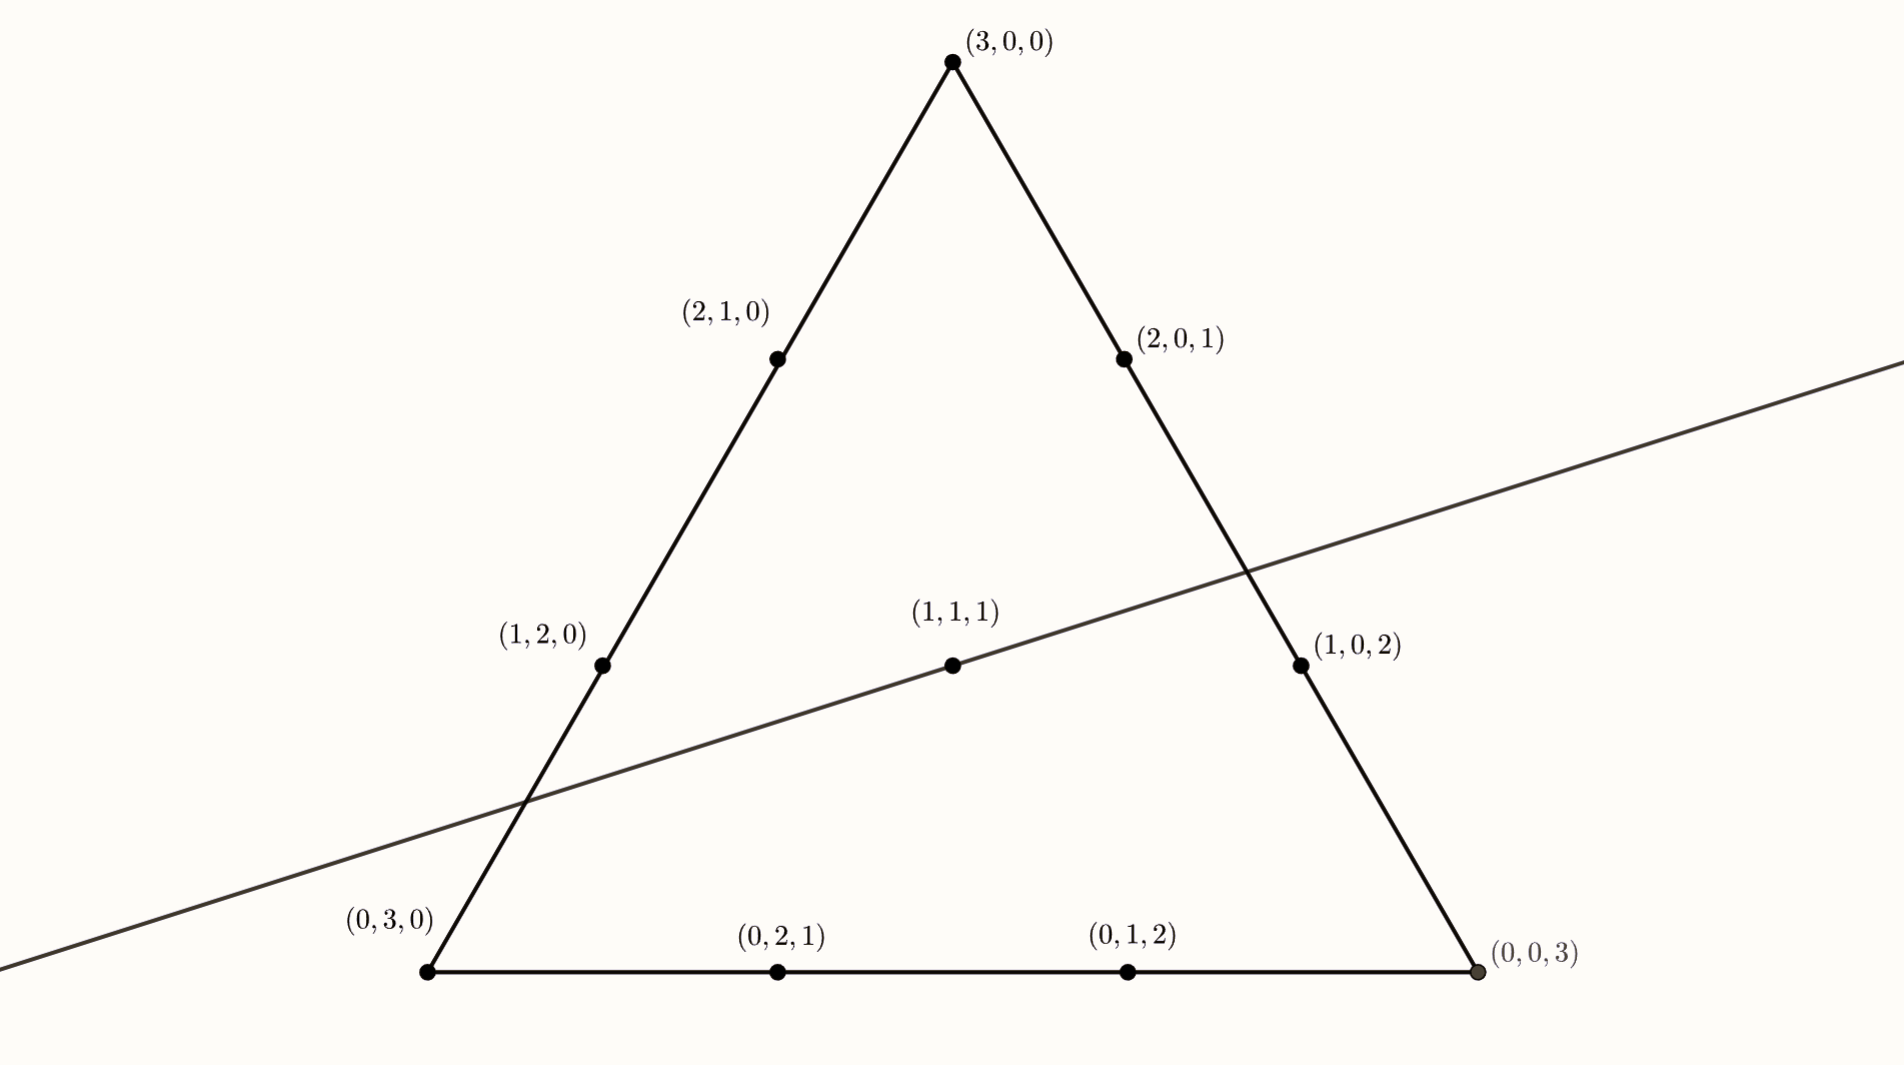
\includegraphics[width=15cm]{1}
    \end{figure}
    The line passing through the triangle is $-7i+2j+5k=0$, and every point above this line has a negative weight and below this line has a positive weight. We conclude this example with the following lemma.
    \begin{lemma}
        A curve of genus one is semi-stable if and only if it has no triple point and no double point with a unique tangent. It is properly stable if and only if it is smooth.
    \end{lemma}
    \begin{proof}
        We know that $\mu(f,\lambda)=\max\{-(3-j-k)a-jb-kc:c_{ijk}\neq 0\}$ where $f$ is the defining polynomial. If $\mu(f,\lambda)<0$ then
        \[c_{300}=c_{210}=c_{201}=c_{120}=c_{111}=0\]
        Conversely, if the above equation is true then take $a=-3$, $b=1$ and $c=2$ we get $\mu(f,\lambda)<0$. Note that the above equation is equivalent to $f$ having a triple point or a double point with a unique tangent. Thus the first claim is proved.

        Now suppose that $f$ has a singular point at $x$. Then we can assume $x=(1,0,0)$ so $c_{300}=c_{210}=c_{201}=0$. If $a=-2$, $b=c=1$ then we have $f$ not properly stable. If $\mu(f,\lambda)\leqslant 0$ for some $\lambda$ then $f$ has a singular point. Indeed, $\mu(f,\lambda)\leqslant 0$ suggests $c_{300}=c_{210}=0$. If $c_{201}=0$ then $(1,0,0)$ is a singular point. If $c_{201}\neq 0$, we have $c-2a\leqslant 0$ which implies $a=b$, $c=-2a$. Thus, $\mu(f,\lambda)=\max\{(3k-3)a\}$ which means $\mu\leqslant0$ if and only if $c_{ij0}=0$ for all $j$, meaning $f=yf'$ for some $f'$ of degree $2$, meaning $f$ is singular at every point of $y=f'=0$ (which is nonempty by Bezout), completing the proof.
    \end{proof}
    \begin{remark}
        The Hilbert-Mumford criterion not only lets us compute the stability of certain points easily, but provides us with some idea of what type of points can be classified/``represented" easily and nicely. For instance, in this example of curves, we realize that smooth curves of genus one modulo isomorphisms have a geometric quotient.
    \end{remark}
    \newpage
    \section{References}
    \nocite{*}
    \renewcommand{\section}[2]{\vskip 0.01em}
    \printbibliography
\end{document}
